% -*- Mode:TeX -*-

%% The documentclass options along with the pagestyle can be used to generate
%% a technical report, a draft copy, or a regular thesis.  You may need to
%% re-specify the pagestyle after you \include  cover.tex.  For more
%% information, see the first few lines of mitthesis.cls. 

%\documentclass[12pt,vi,twoside]{mitthesis}
%%
%%  If you want your thesis copyright to you instead of MIT, use the
%%  ``vi'' option, as above.
%%
%\documentclass[12pt,twoside,leftblank]{mitthesis}
%%
%% If you want blank pages before new chapters to be labelled ``This
%% Page Intentionally Left Blank'', use the ``leftblank'' option, as
%% above. 

\documentclass[12pt,twoside]{mitthesis}
\usepackage{lgrind}
\usepackage[dvips]{graphicx}
\usepackage{verbatim}
\pagestyle{plain}

%% This bit allows you to either specify only the files which you wish to
%% process, or `all' to process all files which you \include.
%% Krishna Sethuraman (1990).

\typein [\files]{Enter file names to process, (chap1,chap2 ...), or `all' to
process all files:}
\def\all{all}
\ifx\files\all \typeout{Including all files.} \else \typeout{Including only \files.} \includeonly{\files} \fi

\begin{document}

% -*-latex-*-
% $Log: not supported by cvs2svn $
% Revision 1.1  2008/08/25 17:36:14  thies
% *** empty log message ***
%
% Revision 1.7  2001/02/08 18:53:16  boojum
% changed some \newpages to \cleardoublepages
%
% Revision 1.6  1999/10/21 14:49:31  boojum
% changed comment referring to documentstyle
%
% Revision 1.5  1999/10/21 14:39:04  boojum
% *** empty log message ***
%
% Revision 1.4  1997/04/18  17:54:10  othomas
% added page numbers on abstract and cover, and made 1 abstract
% page the default rather than 2.  (anne hunter tells me this
% is the new institute standard.)
%
% Revision 1.4  1997/04/18  17:54:10  othomas
% added page numbers on abstract and cover, and made 1 abstract
% page the default rather than 2.  (anne hunter tells me this
% is the new institute standard.)
%
% Revision 1.3  93/05/17  17:06:29  starflt
% Added acknowledgements section (suggested by tompalka)
%
% Revision 1.2  92/04/22  13:13:13  epeisach
% Fixes for 1991 course 6 requirements
% Phrase "and to grant others the right to do so" has been added to
% permission clause
% Second copy of abstract is not counted as separate pages so numbering works
% out
%
% Revision 1.1  92/04/22  13:08:20  epeisach
\title{Language and Compiler Support for Stream Programs}

\author{William Thies}
\department{Department of Electrical Engineering and Computer Science}
% If the thesis is for two degrees simultaneously, list them both
% separated by \and like this:
% \degree{Doctor of Philosophy \and Master of Science}
%\degree{Doctor of Philosophy of Science in Computer Science and Engineering}
\degree{Doctor of Philosophy}
\degreemonth{December} \degreeyear{2008} \thesisdate{\today}

\prevdegrees{~ \\ 
Bachelor of Science, Computer Science and Engineering\\
Massachusetts Institute of Technology, 2001 \\
~ \\
Bachelor of Science, Mathematics\\
Massachusetts Institute of Technology, 2002 \\
~ \\
Master of Engineering, Computer Science and Engineering \\
Massachusetts Institute of Technology, 2002 \\
~ \\
}

%% By default, the thesis will be copyrighted to MIT.  If you need to copyright
%% the thesis to yourself, just specify the `vi' documentclass option.  If for
%% some reason you want to exactly specify the copyright notice text, you can
%% use the \copyrightnoticetext command.
%\copyrightnoticetext{\copyright IBM, 1990.  Do not open till Xmas.}

% If there is more than one supervisor, use the \supervisor command
% once for each.
\supervisor{Saman Amarasinghe}{Associate Professor}

% These are optional, and enabled with reader.sty
%\reader{Arvind}{Professor}
%\reader{Srini Devadas}{Professor}

% This is the department committee chairman, not the thesis committee
% chairman.  You should replace this with your Department's Committee
% Chairman.
\chairman{Terry P. Orlando}{Chair, Department Committee on Graduate Students}

% Make the titlepage based on the above information.  If you need
% something special and can't use the standard form, you can specify
% the exact text of the titlepage yourself.  Put it in a titlepage
% environment and leave blank lines where you want vertical space.
% The spaces will be adjusted to fill the entire page.  The dotted
% lines for the signatures are made with the \signature command.
\maketitle

% The abstractpage environment sets up everything on the page except
% the text itself.  The title and other header material are put at the
% top of the page, and the supervisors are listed at the bottom.  A
% new page is begun both before and after.  Of course, an abstract may
% be more than one page itself.  If you need more control over the
% format of the page, you can use the abstract environment, which puts
% the word "Abstract" at the beginning and single spaces its text.

%% You can either \input (*not* \include) your abstract file, or you can put
%% the text of the abstract directly between the \begin{abstractpage} and
%% \end{abstractpage} commands.

% First copy: start a new page, and save the page number.
\cleardoublepage
% Uncomment the next line if you do NOT want a page number on your
% abstract and acknowledgments pages.
% \pagestyle{empty}
\setcounter{savepage}{\thepage}
\begin{abstractpage}
Due to the high data rates involved in audio, video, and signal
processing applications, it is imperative to compress the data to
decrease the amount of storage used.  Unfortunately, this implies that
any program operating on the data needs to be wrapped by a
decompression and re-compression stage.  Re-compression can incur
significant computational overhead, while decompression swamps the
application with the original volume of data.

In this paper, we present a program transformation that greatly
accelerates the processing of compressible data.  Given a program that
operates on uncompressed data, we output an equivalent program that
operates directly on the compressed format.  Our transformation
applies to stream programs, a restricted but useful class of
applications with regular communication and computation patterns.  Our
formulation is based on LZ77, a lossless compression algorithm
utilized by ZIP, and immediately applies to simpler formats such as
Apple Animation, Microsoft RLE, and Targa.

We implemented a simple subset of our techniques in the StreamIt
compiler, which emits executable plugins for two popular video editing
tools: MEncoder and Blender.  For common operations such as color
adjustment and video compositing, computing directly on compressed
data offers a speedup roughly proportional to the overall compression
ratio.  For our benchmark suite of 12 videos in Apple Animation
format, speedups range from 1.1x to 471x, with a median of 15x.

\end{abstractpage}

% Additional copy: start a new page, and reset the page number.  This way,
% the second copy of the abstract is not counted as separate pages.
% Uncomment the next 6 lines if you need two copies of the abstract
% page.
% \setcounter{page}{\thesavepage}
% \begin{abstractpage}
% Due to the high data rates involved in audio, video, and signal
processing applications, it is imperative to compress the data to
decrease the amount of storage used.  Unfortunately, this implies that
any program operating on the data needs to be wrapped by a
decompression and re-compression stage.  Re-compression can incur
significant computational overhead, while decompression swamps the
application with the original volume of data.

In this paper, we present a program transformation that greatly
accelerates the processing of compressible data.  Given a program that
operates on uncompressed data, we output an equivalent program that
operates directly on the compressed format.  Our transformation
applies to stream programs, a restricted but useful class of
applications with regular communication and computation patterns.  Our
formulation is based on LZ77, a lossless compression algorithm
utilized by ZIP, and immediately applies to simpler formats such as
Apple Animation, Microsoft RLE, and Targa.

We implemented a simple subset of our techniques in the StreamIt
compiler, which emits executable plugins for two popular video editing
tools: MEncoder and Blender.  For common operations such as color
adjustment and video compositing, computing directly on compressed
data offers a speedup roughly proportional to the overall compression
ratio.  For our benchmark suite of 12 videos in Apple Animation
format, speedups range from 1.1x to 471x, with a median of 15x.

% \end{abstractpage}

\cleardoublepage

\newpage
~ \vspace{-3.7\baselineskip}\\
\enlargethispage{0.3\baselineskip}
\section*{Acknowledgments}

I would like to start by expressing my deepest gratitude to my
advisor, colleague and friend, Saman Amarasinghe.
%Saman's committment to me has been downright scary.
%Simply put, Saman has changed my life.
%Simply put, Saman has been the mentor of a lifetime.
From 4am phone calls in Boston to weeks of one-on-one time in Sri
Lanka and India, Saman invested {\it unfathomable} time and energy
into my development as a researcher and as a person.  His extreme
creativity, energy, and optimism (not to mention mad PowerPoint
skills!) have been a constant source of inspiration, and whenever I am
at my best, it is usually because I am asking myself: {\it What would
Saman do}?  Saman offered unprecedented freedom for me to pursue
diverse interests in graduate school -- including weeks at a time
working with other groups -- and served as a fierce champion on my
behalf in every possible way.  I will forever treasure our deep sense
of shared purpose and can only aspire to impact others as much as he
has impacted me.

%Like a Papa Bear, any arguments between the two of us would be 
%completely dwarfed by the fierce battles he would wage on my behalf.

\vspace{-8pt}\paragraph*{Contributors to this dissertation} Many
people made direct contributions to the content of this dissertation.
The StreamIt project was a fundamentally collaborative undertaking,
involving the extended efforts of over 27 people.  I feel very lucky
to have been part of such an insightful, dedicated, and fun team.
Section~\ref{sec:streamit-project} provides a technical overview of
the entire project, including the division of labor.  In what follows
I am listing only a subset of each person's actual contributions.
Michael Gordon, my kindred Ph.D. student throughout the entire
StreamIt project, led the development of the parallelization
algorithms (summarized in Chapter~4), the Raw backend and countless
other aspects of the compiler.  Rodric Rabbah championed the project
in many capacities, including contributions to cache optimizations
(summarized in Chapter~4), teleport messaging (Chapter~3), the MPEG2
benchmarks, an Eclipse interface, and the Cell backend.  Michal
Karczmarek was instrumental in the original language design (Chapter
2) and teleport messaging, and also implemented the StreamIt scheduler
and runtime library.  David Maze, Jasper Lin, and Allyn Dimock made
sweeping contributions to the compiler infrastructure; I will forever
admire their skills and tenacity in making everything work.

Central to the StreamIt project is an exceptional array of
M.Eng. students, who I feel very privileged to have interacted with
over the years.  Andrew Lamb, Sitij Agrawal, and Janis Sermulins led
the respective development of linear optimizations, linear statespace
optimizations, and cache optimizations (all summarized in Chapter~4).
Janis also implemented the cluster backend, with support for teleport
messaging (providing results for Chapter~3).  Matthew Drake
implemented the MPEG2 codec in StreamIt, while Jiawen Chen implemented
a flexible graphics pipeline and Basier Aziz implemented mosaic
imaging.  Daviz Zhang developed a lightweight streaming layer for the
Cell processor; Kimberly Kuo developed an Eclipse user interface for
StreamIt; Juan Reyes developed a graphical editor for stream graphs;
and Jeremy Wong modeled the scalability of stream programs.  Kunal
Agrawal investigated bit-level optimizations in StreamIt.  Ceryen Tan
is improving StreamIt's multicore backend.

The StreamIt project also benefited from an outstanding set of
undergraduate researchers, who taught me many things.  Ali Meli, Chris
Leger, Satish Ramaswamy, Matt Brown, and Shirley Fung made important
contributions to the StreamIt benchmark suite (detailed in Chapter~2).
Steve Hall integrated compressed-domain transformations into the
StreamIt compiler (providing results for Chapter~5).  Qiuyuan Li
worked on a StreamIt backends for Cell, while Phil Sung targeted a
GPU.

%Qiuyuan Li worked on a StreamIt backend for the Cell processor, while
%Phil Sung worked on a backend for graphics processors.

Individuals from other research groups also impacted the StreamIt
project.  Members of the Raw group offered incredible support for our
experiments, including Anant Agarwal, Michael Taylor, Walter Lee,
Jason Miller, Ian Bratt, Jonathan Eastep, David Wentzlaff, Ben
Greenwald, Hank Hoffmann, Paul Johnson, Jason Kim, Jim Psota, Nathan
Schnidman, and Matthew Frank.
%
\newpage
\enlargethispage{0.3\baselineskip}
%
~ \vspace{-1.3\baselineskip}\\
\noindent Hank Hoffmann, Nathan Schnidman, and Stephanie Seneff also
provided valuable expertise on designing and parallelizing signal
processing applications.  External contributors to the StreamIt
benchmark suite include Ola Johnsson, Mani Narayanan, Magnus
Stenemo, Jinwoo Suh, Zain ul-Abdin, and Amy Williams.  Fabrice
Rastello offered key insights for improving our cache optimizations.
Weng-Fai Wong offered guidance on several projects during his visit
to the group.  StreamIt also benefited immensely from regular and
insightful conversations with stakeholders from industry, including
Peter Mattson, Richard Lethin, John Chapin, Vanu Bose, and Andy Ong.

Outside of the StreamIt project, additional individuals made direct
contributions to this dissertation.  In developing our tool for
extracting stream parallelism (Chapter~6), I am indebted to Vikram
Chandrasekhar for months of tenacious hacking and to Stephen McCamant
for help with Valgrind.  I thank Jason Ansel, Chen Ding, Ronny
Krashinsky, Viktor Kuncak, and Alex Salcianu, who provided valuable
feedback on manuscripts that were incorporated into this dissertation.
I am also grateful to Arvind and Srini Devadas for serving on my
committee on very short notice, and to Marek Olszewski for serving as
my remote agent of thesis submission!

\vspace{-8pt}\paragraph*{The rest of the story} Throughout my life,
I have been extremely fortunate to have had an amazing set of
mentors who invested a lot of themselves in my personal growth.  I
thank Thomas ``Doc'' Arnold for taking an interest in a nerdy high
school kid, and for setting him loose with chemistry equipment in a
Norwegian glacier valley -- a tactic which cemented my interest in
science, especially the kind you can do while remaining dry.
%a tactic which ignited not only my interest in science, but also in
%girls.
I thank Scott Camazine for taking a chance on a high school programmer
in my first taste of academic research, an enriching experience which
%was not only enriching and fun, but also 
opened up many doors for me in the future.  I thank Vanessa Colella
and Mitchel Resnick for making my first UROP experience a very
special one, as evidenced by my subsequent addiction to the UROP
program.  I thank Andrew Begel for teaching me many things, not
least of which is by demonstration of his staggering commitment,
capacity, and all-around coolness in mentoring undergraduates.  I'm
especially grateful to Brian Silverman, a mentor and valued friend
whose unique perspectives on everything from Life in StarLogo to
life on Mars have impacted me more than he might know.  I thank
Markus Zahn for excellent advice and guidance, both as my
undergraduate advisor and UROP supervisor.  Finally, I'm very
grateful to Kath Knobe, who provided unparalleled mentorship during
my summers at Compaq and stimulated my first interest in compilers
research.

Graduate school brought a new set of mentors.  I learned a great
deal from authoring papers or proposals with Anant Agarwal, Srini
Devadas, Fredo Durand, Michael Ernst, Todd Thorsen, and
Fr\'{e}d\'{e}ric Vivien, each of whom exemplifies the role of a
faculty member in nurturing student talent.  I am also very grateful
to Srini Devadas, Martin Rinard, Michael Ernst, and Arvind for being
especially accessible as counselors, showing interest in my work and
well-being even in spite of very busy schedules.  I could not have
imagined a more supportive environment for graduate study.

I thank Charles Leiserson and Piotr Indyk for teaching me about
teaching itself.  I will always remember riding the T with Charles
when a car full of Red Sox fans asked him what he does for a living.
Imagining the impressive spectrum of possible replies, I should not
have been surprised when Charles said simply, ``I teach''.  Nothing
could be more true, and I feel very privileged to have been a TA in
his class.

I'd like to thank my collaborators on projects other than StreamIt,
for enabling fulfilling and fun pursuits outside 
% the work described in 
of this dissertation.  In the microfluidics lab, I thank
J.P. Urbanski for many late nights ``chilling at the lab'', his
euphemism for a recurring process whereby he manufactures chips and
I destroy them.  His knowledge, determination, and overall good
nature are truly inspiring.  I also learned a great deal from David
Craig, Mats Cooper, Todd Thorsen, and Jeremy Gunawardena, 
%
\newpage
\enlargethispage{0.5\baselineskip}
%
~ \vspace{-1.5\baselineskip}\\
\noindent who were extremely supportive of our foray into
microfluidics.  I thank Nada Amin for her insights, skills, and
drive in developing our CAD tool, and for being an absolute pleasure
to work with.

%In the microfluidics lab, I learned an immense amount from
%J.P. Urbanski, microfluidic wizard extraordinaire whose work ethic
%is as intense as it is understated -- never again will I think
%lightly of a late night ``chilling at the lab''.

I'm very thankful to my collaborators in applying technology towards
problems in socio-economic development, from whom I've drawn much
support.  First and foremost is Manish Bhardwaj, whose rare
combination of brilliance, determination, and selflessness has been
a deep inspiration to me.  I also thank Emma Brunskill, who has been
a tremendous collaborator on many fronts, as well as
%whose independence and resourcefulness are always humbling.  
%I'm very grateful to Emma Brunskill, Somani Patnaik, 
Sara Cinnamon, Goutam Reddy, Somani Patnaik and Pallavi Kaushik for
being incredibly talented, dedicated, and fun teammates.
%I thank the Venerable Tenzin Priyadarshi and Scott Kennedy for
%valuable support and guidance.
%
%Further in the past, 
I am very grateful to Libby Levison for involving me in my first
project at the intersection of technology and development, without
which I might have gone down a very different path.  I also thank
Samidh Chakrabarti for being a great officemate and friend, and my
first peer with whom I could investigate this space together.

I am indebted to the many students and staff who worked with me on
the TEK project, including Marjorie Cheng, Tazeen Mahtab, Genevieve
Cuevas, Damon Berry, Saad Shakhshir, Janelle Prevost, Hongfei Tian,
Mark Halsey, and Libby Levison.  I also thank Pratik Kotkar,
Jonathan Birnbaum, and Matt Aasted for their work on the Audio Wiki.
I would not have been able to accomplish nearly as much without the
%continuous 
insights, dedication, and hard work of all these individuals.

% leaving out sri lanka guys, since it's not released:
% - Thayaparan Kailainathan
% - Mahendrakumar Senthivel
% - Thayarupan Rajendram
%
% leaving out some TEK authors who I don't even know:
% - Alexandro Artola
% - Binh D. Vo
% - Yuliya Litvak
% - Sheldon Chan
% - Sid Henderson

Graduate school would be nothing if not for paper deadlines, and I
feel very lucky to have been down in the trenches with such bright,
dependable, and entertaining co-authors.  Of people not already cited
as such, I thank Marten van Dijk, Blaise Gassend, Andrew Lee, Charles
W. O'Donnell, Kari Pulli, Christopher Rhodes, Jeffrey Sheldon, David
Wentzlaff, Amy Williams, and Matthias Zwicker for some of the best
end-to-end research experiences I could imagine.

Many people made the office a very special place to be.  Mary McDavitt
is an amazing force for good, serving as my rock and foundation
throughout many administrative hurricanes; I can't thank her enough
for all of her help, advice, and good cheer over the years.  I'm also
very grateful to Shireen Yadollahpour, Cornelia Colyer, and Jennifer
Tucker, whose helpfulness I will never forget.  Special thanks to
Michael Vezza, system administrator extraordinaire, for his extreme
patience and helpfulness in tending to my every question, and fixing
everything that I broke.

I thank all the talented members of the Commit group, and especially
the Ph.D. students and staff -- Jason Ansel, Derek Bruening, Vikram
Chandrasekhar, Gleb Chuvpilo, Allyn Dimock, Michael Gordon, David
Maze, Michal Karczmarek, Sam Larsen, Marek Olszewski, Diego Puppin,
Rodric Rabbah, Mark Stephenson, Jean Yang, and Qin Zhao.  On top of
tolerating {\it way} more than their fair share of StreamIt talks,
they offered the best meeting, eating, and traveling company ever.  I
especially thank Michael Gordon, my officemate and trusted friend, for
making 32-G890 one of my favorite places -- I'm really going to miss
our conversations (and productive silences!)

I'd like to extend special thanks to those who supported me in my job
search last spring.  I feel very grateful for the thoughtful counsel
of dozens of people on the interview trail, and especially to a few
individuals (you know who you are) who spent many hours talking to me
and advocating on my behalf.  This meant a great deal to me.  I also
thank Kentaro Toyama and others at MSR India for being very flexible
with my start date, as the submission of this thesis was gradually
postponed!

I am extremely fortunate to have had a wonderful support network to
sustain me throughout graduate school.  To the handful of close
friends who joined me for food, walks around town, or kept in touch
from a distance: thank you for seeing me through the thick and thin.
I'd like to especially call out to David Wentzlaff, Kunal Agrawal,
Michael Gordon and Cat Biddle, who held front-row season tickets to my
little world and made it so much better by virtue of being there.

Finally, I would like to thank my amazingly loving and supportive
parents, who have always been 100\% behind me no matter where I am
in life.  I dedicate this thesis to them.

%% \clearpage
%% ~ \\ \vspace{1.1in} ~ \\
%% \begin{center}
%% {\bf \large Relation to Prior Publications}
%% \end{center}
\section*{Relation to Prior Publications}
This dissertation alternately extends and summarizes prior
publications by the author.  Chapters 1 and 2 are significantly more
detailed than prior descriptions of the StreamIt
language~\cite{thies-cc02,thies-can02,amarasinghe-ijpp05} and include
an in-depth study of the StreamIt benchmark suite that has yet to be
published elsewhere.  Chapter~3 subsumes the prior description of
teleport messaging~\cite{thies-ppopp05}, including key changes to the
semantics and the first uniprocessor scheduling algorithm.  Chapter~4
is a condensed summary of prior
publications~\cite{gordon-asplos02,lamb-pldi03,agrawal-cases05,sermulins-lctes05,gordon-asplos06},
though with new text that often improves the exposition.  Chapter~5
subsumes the prior report on compressed-domain
processing~\cite{thies07compression}, offering enhanced functionality,
performance, and readability.  Chapter~6 is very similar to a recent
publication~\cite{thies-micro07}.  Some aspects of the author's work
on StreamIt are not discussed in this
dissertation~\cite{karczmarek-lctes03,chen-graphics05}.

Independent publications by other members of the StreamIt group are
not covered in this
dissertation~\cite{kuo05,drake-ipdps06,zhang_lightweight_2007}.  In
particular, the case study of implementing MPEG2 in StreamIt provides
a nice example-driven exposition of the entire
language~\cite{drake-ipdps06}.

%\vspace{1in}
%\begin{center}
%{\bf \large Funding Acknowledgment}
%\end{center}
\section*{Funding Acknowledgment}
This work was funded in part by the National Science Foundation
(grants EIA-0071841, CNS-0305453, ACI-0325297), DARPA (grants
F29601-01-2-0166, F29601-03-2-0065), the DARPA HPCS program, the MIT
Oxygen Alliance, the Gigascale Systems Research Center, Nokia, and a
Siebel Scholarship.
\clearpage

% NOT ACKNOWLEDGING:
%
% - Meha Senthil?
%
% StreamIt:
% - Vijay Saraswat
% - Ryan Newton
% - Ken Steele provided an IPAQ for some of the experiments in Chapter~4.
%
% Teaching:
% - David Liben Nowell
% 
% Microfluidics:
% - natalie andrew
%
% IIH:
% - Seema Kacker
% - Sourav Dey
% - Ajit Dash
% - Alex Krull
% - Oliver Venn
% - Jessica Leon
% - Nikhil Nadkarni
% - Catherine Dunn
%
% All these details:
%
% I am indebted to many additional students and collaborators who
% helped to pursue goals at the intersection of technology and
% development in my graduate school career.
%
% For external contributions to TEK, from Elsevier I thank Ammy
% Votglander, Craig Scott, Jeremy Alder, Spencer de Groot, and
% Christian Pruvost; from First Mile Solutions, I thank Rich
% Fletcher, Amir Alexander Hasson, and Olufemi Omojola; from the
% People's First Network, I thank David Leeming.  
%
% At Innovators In Health, I thank Manish Bhardwaj, Sara Cinnamon,
% Goutam Reddy, Emma Brunskill, Somani Patnaik, Pallavi Kaushik,
% Seema Kacker, Sourav Dey, Ajit Dash, Alex Krull, Oliver Venn,
% Jessica Leon, Nikhil Nadkarni, and Catherine Dunn.  
%
% I also thank Rich Fletcher, Michael Gordon, Jonathan Jackson,
% Jhonatan Rotenberg, Luis Sarmenta, Ammy Votglander for many
% conversations benefiting this research.  I would not have been
% able to accomplish nearly as much without the steadfast
% dedication and help of all of these individuals.


%%%%%%%%%%%%%%%%%%%%%%%%%%%%%%%%%%%%%%%%%%%%%%%%%%%%%%%%%%%%%%%%%%%%%%
% -*-latex-*-

\pagestyle{plain}
  % -*- Mode:TeX -*-
%% This file simply contains the commands that actually generate the table of
%% contents and lists of figures and tables.  You can omit any or all of
%% these files by simply taking out the appropriate command.  For more
%% information on these files, see appendix C.3.3 of the LaTeX manual. 
\tableofcontents
\newpage
\listoffigures
\newpage
\listoftables


\section{Introduction}

Multicore architectures have become the rule rather than the exception in the changing computing landscape. With single-core performance limited by power consumption, memory latency, and circuit complexity, almost all new architectures (certain mobile and embedded applications excepted) are branching into more cores rather than better cores. Exploiting parallelism has already become absolutely critical if applications wish to make full use of current and future architectures.

Compilers for traditional imperative languages are faced with a daunting task when attempting to aid the programmer in this regard: it is very difficult to automatically extract parallelism from a sequential program written in a low-level language such as C. Much of the time, the task of parallelizing a program remains in the hands of the programmer, who must manually convert a single-threaded sequential program into a multithreaded parallel one. While doing so, he must contend with issues specific to the architecture he is targeting, limiting portability, and worry about introducing race conditions or other bugs that typically plague multithreaded programs. Programmers do have access to a number of frameworks such as MPI and OpenMP; however, parallelization of sequential programs remains a difficult process.

The Cell architecture is a novel multicore architecture that differs significantly from traditional SMP architectures: it is both a heterogeneous architecture and one that does \emph{not} use shared memory. Compared to traditional SMP architectures, the design of Cell is a trade-off for computing power, ease of manufacture, and low power consumption at the cost of programming complexity. To a programmer writing an application that runs on Cell, this only leaves him with additional complications.

Streaming languages such as StreamIt~\cite{asplos02} provide a way to alleviate the burden of manually parallelizing applications. In a streaming language, the programmer defines actors that operate on streams of data; the programmer then composes actors and streams into the program. The structure that is explicitly expressed by a streaming language exposes rather than hides the parallelism present in a program, making it much easier for the compiler to automatically extract parallelism. For the programmer, many applications fit within the streaming model, and can be naturally expressed in StreamIt or other streaming languages.

Ideally, a compiler for a streaming language would like to be able to focus on high-level scheduling issues: finding parallelism and scheduling actors to obtain the best possible utilization of available computation resources. However, when presented with a heterogeneous, distributed-memory architecture like Cell, the compiler must instead first contend with numerous low-level issues.

The goal of this thesis is to create a runtime framework for streaming applications on the Cell architecture. The framework is geared towards compilers rather than programmers. Just as a programmer manually parallelizing a sequential program has access to frameworks like MPI that abstract certain low-level operations, the goal of the streaming framework for Cell is to provide similar functionality to streaming language compilers and schedulers that target the Cell architecture.

To this end, this thesis contributes the following:
\begin{enumerate}
\item A runtime library that provides compilers with higher-level primitives than bare Cell hardware.
\item A dynamic scheduler implemented on top of the runtime library that dynamically schedules a stream graph.
\item An analysis of the amount of code required when a compiler or programmer targets the library compared to Cell hardware directly. The library is shown to significantly simply scheduler implementation without adding significant overhead.
\end{enumerate}

The runtime library and dynamic scheduler were designed with the StreamIt language and the StreamIt compiler explicitly in mind. StreamIt constructs and execution patterns map naturally to the framework; however, the framework is general enough that it should also be able to accommodate other streaming languages.

Chapters~2 presents basic background information and related work on streaming languages and parallelization frameworks, and describes the StreamIt language and the Cell architecture in detail. Chapter~3 presents the runtime library along with a discussion of design decisions and implementation issues. Chapter~4 describes how common scheduling patterns a compiler or programmer might generate can be mapped to the library, and compares code complexity and flexibility to programming for Cell directly. Chapter~5 discusses the dynamic scheduler. Chapter~6 gives a brief analysis of the performance of the framework on a test benchmark. Chapter~7 concludes with a discussion of future work and extensions.

\chapter{Background Information}

\section{The StreamIt Programming Language}

    StreamIt is a programming language specifically tailored to DSP
streaming applications. The user creates a graph composed of four
types of StreamIt constructs: \textit{filters},
\textit{pipelines}, \textit{splitjoins}, and \textit{feedback
loops}. Filters encapsulate the computation done within an
application - they represent the blocks mentioned in the previous
chapter. Each filter operates on a one-dimensional `tape' of
values (of any type, including structures and arrays).  The other
three constructs dictate the type of connections possible between
filters. Every construct explicitly states its input type and
output type, and can be passed parameters as would be to a
procedure.

    StreamIt uses a buffer between every pair of filters to
hold values. When the input buffer of a construct (equivalent to
the output buffer of the previous construct) is appropriately
filled, the construct can execute. Execution involves three steps:
reading and removing items from the input buffer (consumption);
performing computations; putting items in the output buffer
(production). We will not consider the intricacies of managing
these buffers, and instead refer to the more abstract notion of a
tape.

    A filter has pre-defined \textit{peek}, \textit{pop}, and
\textit{push} rates (StreamIt code examples are given below).
During each execution, the filter accesses a maximum of peek
values from its input tape, consumes exactly pop input values from
its input tape, and produces exactly push values onto its output
tape. Since the removal of an input value is technically an access
of that input, the peek rate of a filter must be greater than or
equal to the pop rate of that filter. The push or pop rate can be
zero - the former corresponds to a filter that consumes items but
does not produce them (typically the last filter in a sequence)
and the latter corresponds to a filter that produces items but
does not consume them (typically the first filter in a sequence).
All the accesses, outputs, and removals, as well as all the
computation is done inside the main body of the filter, known as
the work function.

\begin{figure}[bthp]
  \centering
  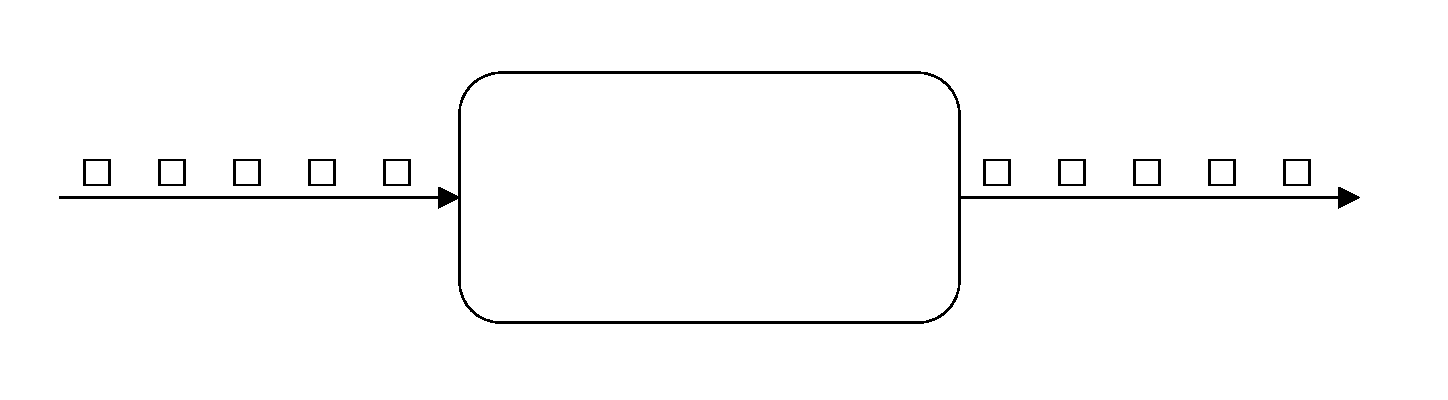
\includegraphics[width=6.0in]{figures/filter.eps}
  \caption{StreamIt filter}
  \label{fig:filter}
\end{figure}

    StreamIt also supports a \textit{prework} function, which has its own push,
pop, and peek rates.  The prework function executes in place of
the work function for the first computation sequence, and is never
run again. Additionally, there is an \textit{init} function which
is run only once upon creation of the filter, and is usually used
to initialize variables.  The init and prework functions are both
optional.

        A filter can store two types of variables - \textit{field} and
\textit{local}. Field variables are declared outside of the
specific functions (work, prework, init), and can be accessed from
anywhere within the filter. Local variables are declared within a
specific function, and only have scope within that function. For
example, a variable declared within the init function is local,
and could not be accessed within the work function. Therefore, the
init function is used to initialize field variables.

Code examples of StreamIt filters are shown below.

\begin{scriptsize}
\begin{verbatim}
// This filter adds the parameter scalar to each input.
// It does not have an init or prework function
float -> float filter scalarAdd(float scalar) {
  work push 1 pop 1 peek 1 {
    push(scalar + pop());
  }
}
\end{verbatim}
\end{scriptsize}

\begin{scriptsize}
\begin{verbatim}
// This filter outputs a running average of every three consecutive inputs.
// The first time it runs, it ouputs the average of the first two inputs without removing anything from the tape.
// It does not have an init function.
float -> float filter threeWayAverage() {
  prework push 1 pop 0 peek 2 {
    float temp;  // example of a local variable
    temp = (peek(0)+peek(1))/2;
    push(temp);
  }
  work push 1 pop 1 peek 3 {
    float temp;  // example of a local variable
    temp = (peek(0) + peek(1) + peek(2))/3
    push(temp);
    pop()
  }
}
\end{verbatim}
\end{scriptsize}

\begin{scriptsize}
\begin{verbatim}
// This filter computes an infinite impulse response function.
// It does not have a prework function.
float->float filter IIR() {
    float curr;  // example of a field variable
    init {
      curr = 0;
    }
    work push 1 pop 1 peek 3 {
      float temp;  \\ example of a local variable
      temp = (peek(0) + peek(1) + peek(2))/6;
      curr = temp + curr/2;
      push(curr);
      pop();
    }
}
\end{verbatim}
\end{scriptsize}

    Pipelines, splitjoins, and feedback loops are higher level
constructs created from filters. Each structures the layout of its
filters in a certain format. Even though these three constructs do
not directly provide the syntax to perform computations and work
from an input or output tape, they can be thought of as filters in
the following way: the construct recieves inputs which are passed
to one or more of the filters; all the filters perform
computations and pass values to one another through their input
and output tapes; the construct outputs values from one or more of
its filters. In fact, for every pipeline, splitjoin, and feedback
loop there is an equivalent filter representation. Therefore,
these three constructs are not strictly necessary for writing a
StreamIt program. However, they simplify and structure writing a
large application.

    The higher level constructs are not limited to combine filters -
they can also combine each other. This follows directly from the
fact that a higher level construct has some equivalent filter.
Therefore, if a pipeline can be composed of filters, it can also
be composed of pipelines, splitjoins, and feedback loops, which
are all like filters. We shall refer to all four StreamIt
constructs generically as blocks. This corresponds to the fact
that any StreamIt construct behaves as a block: it takes inputs,
performs calculations, and produces outputs.

    Pipelines combine a set of blocks in sequential fashion, so that
the output of the first block is the input to the second block,
the output of the second block is the input to the third block,
etc. The blocks are placed in order using the add statement.

\begin{figure}[bthp]
  \centering
  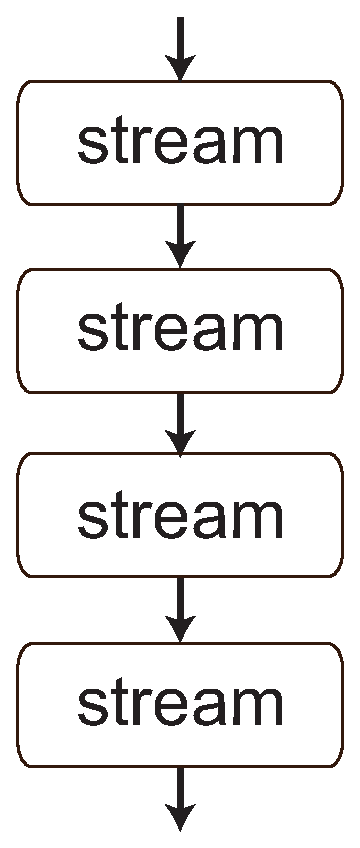
\includegraphics[width=6.0in]{figures/pipeline.eps}
  \caption{StreamIt pipeline}
  \label{fig:pipeline}
\end{figure}

\begin{scriptsize}
\begin{verbatim}
// This pipeline connects the filters scalarAdd and threeWayAverage.
// The parameter scalar passed to this pipeline is passed to the
// filter scalarAdd.
float -> float pipeline combinedWork(float scalar) {
  add scalarAdd(scalar);
  add threeWayAverage();
}
\end{verbatim}
\end{scriptsize}

    A splitjoin arranges blocks in a parallel fashion.  The inputs to
a splitjoin are sent to each block in a \textit{roundrobin} or
\textit{duplicate} manner, and the outputs of each block are
joined in a roundrobin manner. Duplicate splitting means the
inputs to the splitjoin are copied and sent to each block, so that
each block receives exactly the same set of inputs.  Roundrobin
splitting means the inputs to the splitjoin are sent to each block
according to user defined weights.  For example, the first block
receives two inputs, the second block receives one input, the
third block receives two inputs.  Therefore, each block sees a
different set of inputs. Roundrobin joining (the only type of
joining permitted) means the outputs of each block are combined
according to user defined weights, and these represent the outputs
of the entire splitjoin. Blocks are listed in the order which they
recieve inputs using add statements. The way inputs are sent is
determined by using the split statement before the block list, and
the way outputs are recieved is determined by using the join
statement after the block list.

\begin{figure}[bthp]
  \centering
  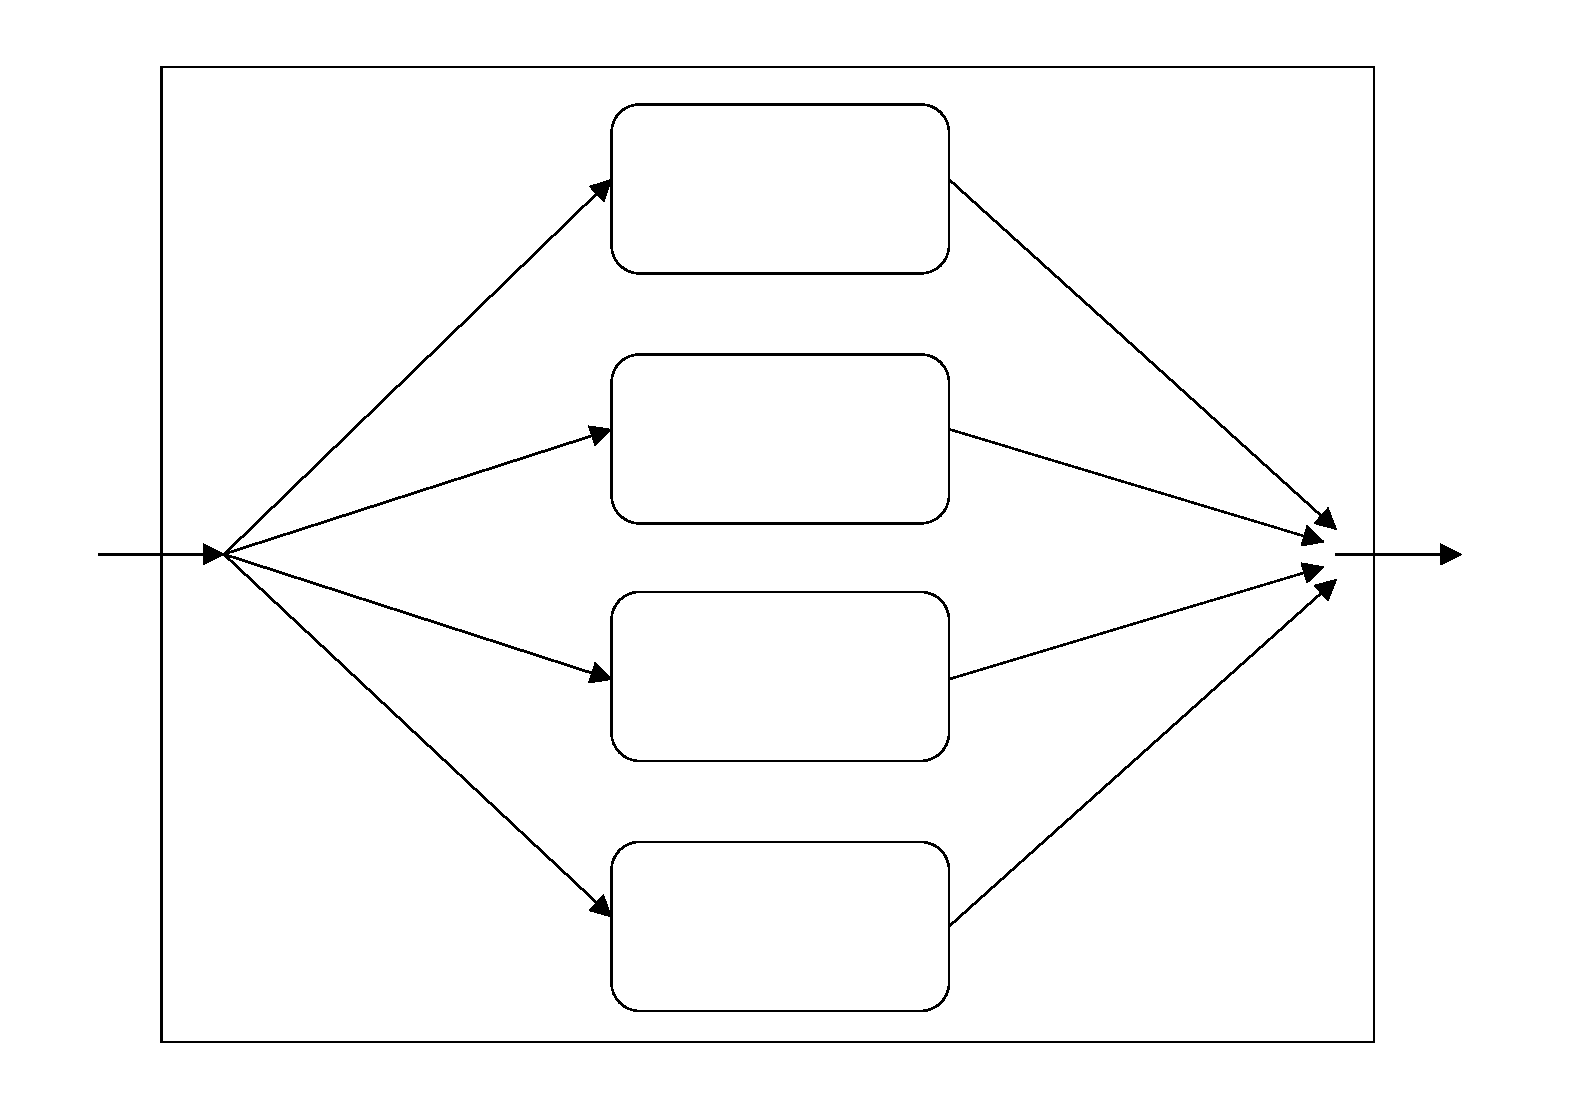
\includegraphics[width=6.0in]{figures/splitjoin.eps}
  \caption{StreamIt splitjoin}
  \label{fig:splitjoin}
\end{figure}

\begin{scriptsize}
\begin{verbatim}
// This splitjoin splits its inputs three ways.
// The first two inputs are sent to the first block, the next
// input to the second block, and the next two inputs to the third
// block.
// The outputs are collected in the following manner: three from
//the first block, five from the second block, and four from the
// third block.
// For every 2+1+2=5 values inputted, 3+5+4=12 values are
// outputted.
float -> float splitjoin mySplitjoin() {
 split roundrobin(2,1,2);
  add combinedWork(3.5);
  add combinedWork(4.5);
  add threeWayAverage();
join roundrobin(3,5,4);
}
\end{verbatim}
\end{scriptsize}

    A feedback loop uses some of its output as
an input. It consists of a body block and a loop block. The input
to the entire feedback loop is combined with the output of the
loop block and sent to the body block, via a roundrobin joiner.
The output of the body block is split two ways in a roundrobin or
duplicate manner.  The first set of outputs is used as the output
of the entire feedback loop, and the second set of outputs is used
as the input to the loop block. Note that there must be initial
values enqueued on the output tape of the loop block in order for
the feedback loop to begin executing. The first statement in a
feedback loop is a join, determining how inputs are sent to the
body block. The body and loop blocks are listed next. The last
statement is a split, determining where outputs are sent from the
loop block.

\begin{figure}[bthp]
  \centering
  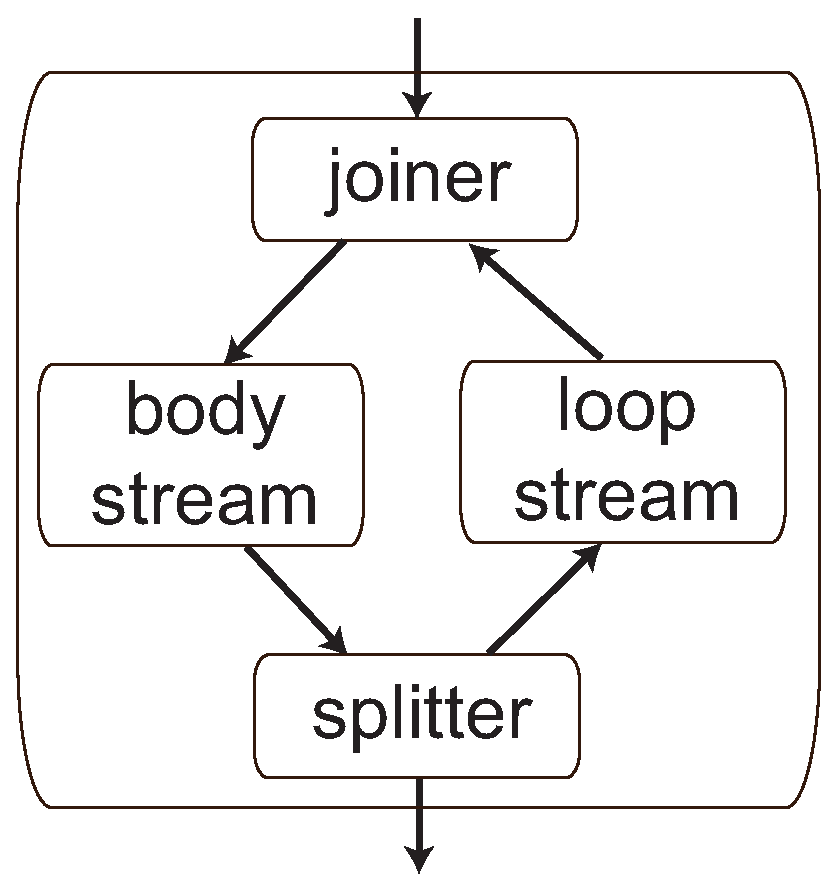
\includegraphics[width=6.0in]{figures/feedback.eps}
  \caption{StreamIt feedback loop}
  \label{fig:feedback}
\end{figure}

\begin{scriptsize}
\begin{verbatim}
// This is a feedback loop implementation of the IIR filter.
// The body and loop are both anonymous filters.
float -> float feedbackloop IIRFeedback() {
  join roundrobin(3,1);
  body float->float filter {
    work push 1 pop 1 peek 4 {
      push((peek(0)+peek(1)+peek(2))/6 + peek(3)/2);
      pop();
    }
  };
  loop float->float filter {
    work push 1 pop 1 peek 1 {
      push(pop());
    }
  };
  split duplicate();
  enqueue(0.0);
}
\end{verbatim}
\end{scriptsize}

    To run a program, the StreamIt compiler finds a
steady-state schedule of the number of times to execute each
filter \cite{Karczmarek}. If such a schedule cannot be found, the
user created block diagram is ill-formed and could not represent a
real world application.

\section{Block Representations}

    The execution of a block (StreamIt or otherwise) can by
characterized by a single equation if the block is linear, and a
pair of equations if the block is state-space linear. We describe
these terms in detail below.

\subsection{Linear Representations}

    A block is termed linear if its outputs are a linear
combination of its inputs plus a set of constants. In mathematical
terms, this relationship can be modelled by the equation
$\vec{\mathbf{y}} = \mathbf{D}\vec{\mathbf{u}} +
\vec{\mathbf{b}}$, where $\vec{\mathbf{u}}$ is a column vector
representing the inputs, $\mathbf{D}$ is a matrix representing the
weights applied to each input, $\vec{\mathbf{b}}$ is a column
vector representing constants added to the inputs, and
$\vec{\mathbf{y}}$ is a column vector representing the outputs.

    Suppose we have the following linear model:
\begin{eqnarray*}
\vec{\mathbf{y}} = \left [ \begin{array} {cc} 1 & 2 \\ 3 & 4 \\
5 & 6 \end{array} \right ] \vec{\mathbf{u}} + \left [
\begin{array} {c} 7
\\ 8 \\ 9 \end{array}\right ]
\end{eqnarray*}

    It is exactly described by the following StreamIt filter:
\begin{scriptsize}
\begin{verbatim}
int -> int filter linearFilter() {
  work push 3 pop 2 peek 2 {
    push(1*peek(0) + 2*peek(1) + 7);
    push(3*peek(0) + 4*peek(1) + 8);
    push(5*peek(0) + 6*peek(1) + 9);
    pop(); pop();
  }
}
\end{verbatim}
\end{scriptsize}

    A process for analyzing and optimizing linear StreamIt filters
is described in \cite{Lamb}.

\subsection{State-Space Representations}

    A more general way of representing a block is by a state-space model.
A set of variables captures the `state' of the filter, so that the
output is a combination of these variables (termed state
variables) and the inputs. Additionally, the states themselves
change upon every execution of the block. This is represented by
the two equations:
\begin{eqnarray*}
\vec{\mathbf{y}} & = & g(\vec{\mathbf{x}},\vec{\mathbf{u}}) \\
\vec{\dot{\mathbf{x}}} & = & f(\vec{\mathbf{x}},\vec{\mathbf{u}})
\end{eqnarray*}

    The state vector is denoted by $\vec{\mathbf{x}}$, the inputs by $\vec{\mathbf{u}}$,
and the outputs by $\vec{\mathbf{y}}$. $\vec{\dot{\mathbf{x}}}$
represents the new state vector, i.e. the state vector after it is
updated. The first equation is for the outputs, the second
equation is for the state updates.

    A linear state-space model has the additional property that
the state updates and outputs are linear in the state variables
and inputs. We can use a simpler set of equations:
\begin{eqnarray*}
\vec{\mathbf{y}} & = & \mathbf{C}\vec{\mathbf{x}}  +
\mathbf{D}\vec{\mathbf{u}} \\
\vec{\dot{\mathbf{x}}} & = & \mathbf{A}\vec{\mathbf{x}} +
\mathbf{B}\vec{\mathbf{u}}
\end{eqnarray*}

    $\mathbf{A}$, $\mathbf{B}$, $\mathbf{C}$, and $\mathbf{D}$ are
matrices whose dimensions depend on the number of states, inputs,
and outputs. Not all blocks can be represented by a linear
state-space model. However, a linear state-space model is more
general than a linear model, so a wider class of blocks can be
represented. We will not discuss general state-space models any
further in this paper, therefore we will write state-space instead
of linear state-space for conciseness.

    Suppose we have the following state-space model:
\begin{eqnarray*}
\vec{\mathbf{y}} & = & \left [ \begin{array} {cc} 11 & 12
\end{array} \right ] \vec{\mathbf{x}} + \left [ \begin{array} {ccc} 13 & 14 & 15 \end{array} \right
 ] \vec{\mathbf{u}} \\
\vec{\dot{\mathbf{x}}} & = & \left [ \begin{array} {cc} 1 & 2 \\ 6
& 7 \end{array} \right ] \vec{\mathbf{x}} + \left [ \begin{array} {ccc} 3 & 4 & 5 \\
8 & 9 & 10 \end{array} \right ] \vec{\mathbf{u}}
\end{eqnarray*}

    It is exactly described by the following StreamIt filter:
\begin{scriptsize}
\begin{verbatim}
int -> int filter stateSpaceFilter() {
  int x1, x2;
  work push 1 pop 3 peek 3 {
    int x1_temp, x2_temp;
    push(11*x1 + 12*x2 + 13*peek(0) + 14*peek(1) + 15*peek(2));
    x1_temp = 1*x1 + 2*x2 + 3*peek(0) + 4*peek(1) + 5*peek(2);
    x2_temp = 6*x1 + 7*x2 + 8*peek(0) + 9*peek(1) + 10*peek(2);
    x1 = x1_temp;
    x2 = x2_temp;
    pop(); pop(); pop();
  }
}
\end{verbatim}
\end{scriptsize}

    Note we introduced two extra variables - $x1\_temp$ and $x2\_temp$.
We do this because we do not want to overwrite the old values for
$x1$ and $x2$ until all the new values are calculated. Also, we
have made no provisions for constants as in the linear model. This
issue is resolved in the next chapter.

\section{The Streaming Runtime Library for Cell}\label{ch:lib}

The Cell architecture provides an excellent target for streaming language compilers for a number of reasons:
\begin{itemize}
\item Individual SPEs are optimized for computation.
\item The limited local store available on SPEs is not a severe limitation for actors in a stream program, which are independent, have extremely local data-access patterns, and generally have small code sizes. In an SDF model such as the basic StreamIt model, known static rates further simplify scheduling.
\item The high-bandwidth, low-latency on-chip communication network enables a large number of scheduling options which would not be feasible for other targets, such as computing clusters.
\end{itemize}

The natural division of work on the Cell architecture maps computation to SPEs, which perform DMA operations to copy input and output data to/from local store. In this model, the PPE functions mainly as a control processor, possibly also performing small amounts of computation that are too small to dispatch to an SPE.

Using this model, a streaming language compiler (or programmer) must address four major issues:
\begin{enumerate}
\item Generating highly-SIMDized code in the limited SPE instruction set. SIMD is required to make full use of an SPE's execution units. In addition, code that operates only on vectors avoids rotate instructions needed to load scalar values from local store, in effect producing a greater performance improvement than would be expected.
\item Generating code that performs DMA operations. This code also needs to double-buffer input and output to make full use of Cell's asynchronous communication model.
\item Organizing all needed code and sufficient buffering to fit into limited SPE local store. This is particularly a problem for larger applications, for which the total code size for all filters leaves little room for buffering, or may exceed the size of local store entirely.
\item Performing high-level optimizations and scheduling. At a high level, compilers would typically be interested in balancing workload among available SPEs, avoiding excess communication, transforming code to improve efficiency, and other such topics.
\end{enumerate}

The purpose of the streaming runtime library for Cell is to abstract \textsf{(2)} and provide facilities that simplify \textsf{(3)} and \textsf{(4)}. The library frees a compiler or programmer from needing to deal with the details of Cell's communication model, allowing it to focus on exploring high-level optimization and scheduling choices. The two main functions of the library are:
\begin{itemize}
\item Providing high-level facilities in place of explicit DMA operations between SPE local stores and memory.
\item Providing the \emph{user}\footnote{\emph{User} refers to all non-library code running on the PPE; typically, most of this performs scheduling. Code for filter work functions and auxiliary functions will always be referred to separately.} with a generic framework for controlling and dispatching computation to SPEs that simplifies scheduling operations.
\end{itemize}

While the library was designed with StreamIt constructs in mind, it is not specific to that language. The library can be used with filters and stream graphs that follow a basic set of specifications, regardless of the original streaming language.

\section{Library Constructs}

The library defines several constructs for the SPEs and PPE. Most facilities provided by the library operate on one or more of these constructs.

\subsection{SPE Constructs: Filters and Buffers}

Two basic constructs are defined for SPEs: \emph{filters} and \emph{buffers}.

\emph{Filters} have similar semantics as StreamIt filters, but are more generalized. A filter represents a generic actor that exposes a work function which is conceptually run infinitely. Filters may be stateful and can read from multiple input tapes and write to multiple output tapes. While a library filter can correspond directly to a single filter in a StreamIt program, a compiler can also perform optimizations, such as fusing multiple StreamIt filters into a single library filter. Work functions are opaque to the library and the library does not perform any SIMDization; that task is left to the compiler or programmer.

\emph{Buffers} are contiguous regions of SPE local store that are reserved for temporarily storing data that is on an input or output tape. All buffers are circular, and the library maintains head and tail pointers for each buffer that indicate where data begins and ends. Conceptually, a buffer has front and back ends; data towards the front of a buffer originated earlier in the execution of the program.

Conceptually, a filter consists of two major components, \emph{code} and \emph{state}, as well as basic properties that describe its work function such as the number of input and output tapes. \emph{Code} is a single contiguous block of arbitrary data that may contain constant data and instructions that define multiple functions; the library only requires that it contain a function with a specific signature, which is used as the work function. Code for a filter is intended to be a single modular component that can be easily relocated to different local store addresses on different SPEs. As such, it should not reference any absolute addresses, such as in absolute branches or loads, or modify itself.\footnote{If the user can accept limitations, such as not being able to relocate filter code or tying code to a single SPE, these suggestions can be ignored.} The latter constraint means that code should not contain any global variables; instead, all global variables should be declared and accessed through fields in the filter's state. \emph{State} contains all mutable data that must be maintained across iterations of the work function. State for different filters is disjoint, and filter code should not access mutable global state. Although a filter's code and state must reside in SPE local store when the filter's work function is running, every filter must have a permanent store for them in memory. The library provides facilities for loading code onto SPEs and copying state between local store and memory.

A filter's work function typically accesses its tapes by reading from the front of its input buffers and writing to the back of its output buffers. This is not enforced by the library and filters can have other data access patterns; however, the library is designed to expect this pattern and the user must take special care otherwise. Filter work functions do not need to have static rates, and the library is agnostic to a filter's rates.

Before a filter can be run on an SPE, it must be loaded onto the SPE through the library. The user provides the library with the properties of the filter and the LS address of its work function; the library initializes a control block that describes the loaded filter in local store, the LS address of which identifies the loaded filter in all future operations. If the filter is stateful, the library also copies its state into local store from its permanent store in memory. Code for the filter must be separately copied into local store through the library, but can be located anywhere as long as the correct work function address is provided to the library. When the user is done with a loaded filter, it can unload the filter through the library, causing the library to copy the filter's state back to its permanent store in memory. Stateful filters can be loaded on at most one SPE at any time, while stateless filters can be simultaneously loaded on any number of SPEs.

This separation of code and state allows the user additional control over how and when SPE local store is used. Since code is constant, the user can preload the code of a filter onto an SPE even while the filter is loaded on another SPE (and thus its state is owned by that SPE) in preparation for loading it on the first SPE in the future. If multiple (possibly stateful) filters have identical code, only one copy of it needs to reside in memory or an SPE's local store and it can be shared. When a filter is not being run, its code does not need to be present in SPE local store, leaving more space free for buffering (local store management is discussed in more detail below).

The library provides similar facilities for allocating buffers on SPEs. The size of a buffer must be a power of two, to allow wrap-around computations to be done with a single \textsf{AND} instruction. Buffers are identified by the LS address that their data region starts at in SPE local store; when allocating a buffer, the library initializes a control block located immediately before the data region that stores the buffer's head and tail pointers and participates in data transfers. As an additional step required before a loaded filter can be run, the user must specify which buffers the filter's input and output tapes refer to.

The library does not provide memory management for SPE local store; when filter code, filter control blocks, and buffers are allocated, the user must manually specify their LS addresses and ensure that the regions used by different constructs do not overlap.\footnote{The library handles all resulting communication, such as copying filter code and state.} This does not create as many difficulties as may appear, as any memory management algorithm that can be implemented internally by the library can just as easily be duplicated by the user on the PPE. Moreover, allowing the user to explicitly manage local store allows it to implement far more complex algorithms as desired. Additionally, in this scheme, buffers and space occupied by filter code and filter control blocks for stateless filters never need to be explicitly deallocated -- the user can simply reuse the local store region for other constructs after it is certain that they are no longer in use.

Theoretically, the number of filters loaded and buffers allocated on an SPE is limited only by available local store. However, there is generally no useful purpose in keeping more than two filters and their associated buffers on an SPE at any time.

\subsection{PPE Constructs}

The library does not define a filter construct for the PPE. However, because all memory is addressable by PPE code, the user can easily create similar behavior.

The library defines a PPE or memory buffer construct that is an extension of the SPE buffer. PPE buffers are not required to be circular, and buffers that are non-circular have no size limitations. PPE buffers are identified by the address of their control block, and multiple buffers can refer to the same data region, with different head and tail pointers. This is used to implement certain StreamIt features with minimal overhead, such as duplicate splitters and data-parallel execution. Because of the limited size of SPE local store, this functionality was considered unnecessary for SPE buffers.

Conceptually, data produced during the execution of a program is contained in exactly one buffer (which may be an SPE or PPE buffer) until it is consumed. The library provides facilities for moving data between buffers on different processors.
 
\section{Library Commands}

Under the library, SPEs only execute library code and filter code. User code on the PPE dispatches work items to SPEs by issuing library \emph{commands}, and is notified when SPEs complete them. Each library command encapsulates a specific action to be performed, and has parameters that are specified by the user. Commands can be divided into three main types:
\begin{itemize}
\item Filter commands: commands to load or unload filters, copy filter code into local store, attach tapes to buffers, and run filters.
\item Buffer commands: commands to allocate buffers.
\item Data transfer commands: commands to move data between buffers in the local stores of different SPEs, or local store and memory.
\end{itemize}

As an example, the \textsf{filter\_run} command, which runs a loaded filter, takes two parameters: the LS address of a loaded filter's control block, and the number of iterations to run the work function for. The user is responsible for ensuring that there is sufficient data in input buffers and sufficient space in output buffers for all specified iterations. Other commands have similar requirements. For a complete description of all commands, see appendix~\ref{app:ui:cmd}.

The amount of work specified by a single command varies depending on parameters to the command. Typically, \textsf{filter\_run} commands do not take more than a few hundred microseconds to complete; some other commands are auxiliary commands and complete almost immediately. This allows the user to quickly change scheduling decisions and avoids tying an SPE into any specific long-term action.

When the user issues a command to an SPE, it assigns the command an ID that must be unique among all commands previously issued to that SPE that have not completed. This ID is used to notify the user when the SPE finishes executing the command. 

\subsection{Dependencies}

In order to keep SPEs supplied with work at all times, it is necessary to limit round-trips between the PPE and SPEs during which the SPEs have no commands to execute. The library provides a general facility for queuing and ordering commands on individual SPEs by allowing each command to specify a set of command IDs on that SPE that it depends on. Commands issued to an SPE are queued and executed only after all dependencies have finished.

At any time, a command that has been issued to an SPE can be either \emph{queued} (a command with unfinished dependencies), \emph{active} (a command with all dependencies satisfied and currently being executed), or \emph{completed} (a command for which all work has been done, but the user has not yet been notified). From the perspective of the user, all commands that are active on an SPE are run ``concurrently''. When a command is issued, all dependency IDs that have not been issued are considered to have already completed and are ignored.

In effect, each SPE maintains a small dependency graph of commands that represents a small subset in time and space of the entire schedule the user executes a program with. User code on the PPE continually adds commands to the dependency graph, while the SPE continually processes commands that have their dependencies satisfied. To make full use of an SPE, it is only necessary for the PPE to ensure the dependency graph on the SPE is never empty. The user cannot remove commands once issued, but if it keeps the dependency graph low-depth, it can quickly change the pattern of work done by an SPE simply by issuing a different set of new commands.

\subsection{Command Groups}

Each command has a small amount of data associated with it, consisting of command-specific parameters in addition to generic ID and dependency information. Typically, the user will be issuing sets of related commands at once. To avoid the overhead of issuing each command individually, the user can organize commands into groups; the library only allows entire command groups to be issued.\footnote{To issue a single command, the user can create a group containing only that command.} Each group specifies a sequence of commands; until a group is explicitly cleared, commands in the group are saved and can be reissued in the future.

Since SPE local store is managed by the user, the user must provide the library with an LS address where command data will be copied to when it issues a command group. For dependency purposes, SPEs treat commands in a group as having been issued in the order they appear in the group. Although commands are issued in groups, the user is notified when individual commands complete.

\subsection{User Interface}

Commands issued to different SPEs are completely independent; the dependency graph on each SPE is strictly local. User code on the PPE thus serves as the main point of synchronization between SPEs by adjusting the commands it issues to an SPE in response to command completion notifications from all SPEs.

User code on the PPE is mainly callback-driven. The user registers a callback function with the library that is called whenever a command issued to an SPE completes. The library maintains a per-SPE bitmap of command IDs that have completed; the user can query this bitmap in the callback to determine which commands have completed and respond accordingly. Bits in the bitmap are set until explicitly acknowledged by the user. After an ID has been acknowledged, it can be reused for new command issued to the SPE.

The library does not maintain a dependency graph on the PPE. Some SPE commands have equivalents on the PPE provided as library functions, which are run immediately when called.

Appendix~\ref{app:ui} contains complete specifications for the interface provided by the library to user code.

\subsection{Data Transfer}

Data transfer commands indirectly result in additional points of synchronization between processors. A data transfer conceptually moves data from the front of a source buffer to the back of a destination buffer, and requires two commands: a command to transfer data out of the source buffer, issued to the processor containing the source buffer, and a command to transfer data into the destination buffer, issued to the processor containing the destination buffer. Where either buffer is located in memory, the user instead calls a library function.

Splitting data transfers into a pair of commands with one on each processor provides the user with explicit control over when the data transfer occurs with respect to both processors. The library ensures that the transfer does not occur until both commands become active on their respective processors. The user must ensure, via the dependency graphs on SPEs or manually on the PPE, that when a data transfer command becomes active on a processor, the local buffer has sufficient data or space to fulfill the transfer.

Data transfers impose minor alignment requirements on the buffers involved due to limitations of Cell's underlying DMA model. There are no restrictions on the size of a data transfer (except for the size of the buffers involved), but the same size must be specified by both commands in the pair. Each data transfer command also specifies the address and size of the opposing buffer, since this is information the user will know in advance; however, buffer head and tail pointers, which are more difficult to track in advance, are handled by the library. In addition, data transfer commands have additional inter-SPE requirements that the user must ensure are met across all SPEs. When a data transfer command becomes active on an SPE, the opposing buffer must already be allocated on the opposing SPE. As well, for any buffer, at most one data transfer in command and one data transfer out command specifying it as the opposing buffer can be active at any time across all processors.

This ``decoupling'' of data transfers simplifies the information the user needs to keep track of. When issuing commands to one SPE, the user usually does not need to be concerned with the state of other SPEs; as long as pairs of data transfer commands are eventually issued with the correct parameters and dependencies, the library will handle synchronization between buffers.

\section{Filter Code}

The interface provided by the library for writing filter code consists of a set of C header files that define a collection of preprocessor macros that simplify state and tape access. StreamIt code can be converted almost directly to code for a library filter. For complete specifications, see appendix~\ref{app:filterui}.

\section{User Code Examples}

As an example, we will illustrate the commands required to set up and run a sample filter on an SPE. For simplicity, this filter has a single input tape, single output tape, and static rates: its work function pops $i$, peeks $i+e$, and pushes $o$ bytes per iteration.

Before the filter can be run, it must be loaded, its input and output buffers must allocated, and the filter's tapes must be attached to the buffers. The commands that perform this are illustrated in figure~\ref{fig:lib:init}.

\begin{figure}[!htb]
\begin{center}
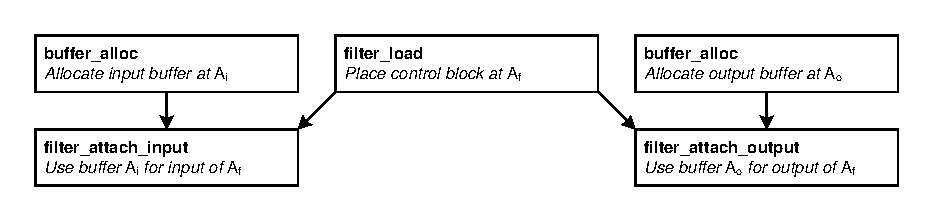
\includegraphics{figs/init}
\end{center}
\caption[Commands to set up a filter.]{Commands to load a filter and allocate and attach input and output buffers. Lines between commands represent dependencies that must be specified to the library when the commands are issued. These commands may be issued in one or multiple groups. See appendix~\ref{app:ui} for detailed information on setting up commands and dependencies.}
\label{fig:lib:init}
\end{figure}

In addition, input data must be transferred into the input buffer before the filter can be run, and output data must eventually be transferred out of the output buffer. With an initially empty input buffer, the commands to transfer in $n$ iterations of input, run the filter for $n$ iterations, and then transfer out $n$ iterations of output (assuming that the input and output buffers were sized appropriately) are shown in figure~\ref{fig:lib:run}.

\begin{figure}[!htb]
\begin{center}
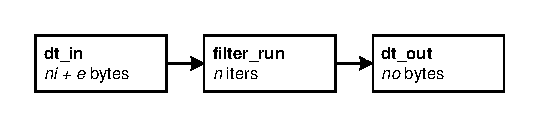
\includegraphics{figs/run}
\end{center}
\caption[Commands to run a filter.]{Commands to run a filter for the first $n$ iterations, including transferring input and output. The corresponding data transfer commands on other SPEs or the PPE are not shown.}
\label{fig:lib:run}
\end{figure}

To run the filter for a larger number of iterations, a sequence of commands is required due to the limited buffer space available in SPE local store. This is illustrated in figure~\ref{fig:lib:ext}.

\begin{figure}[!htb]
\begin{center}
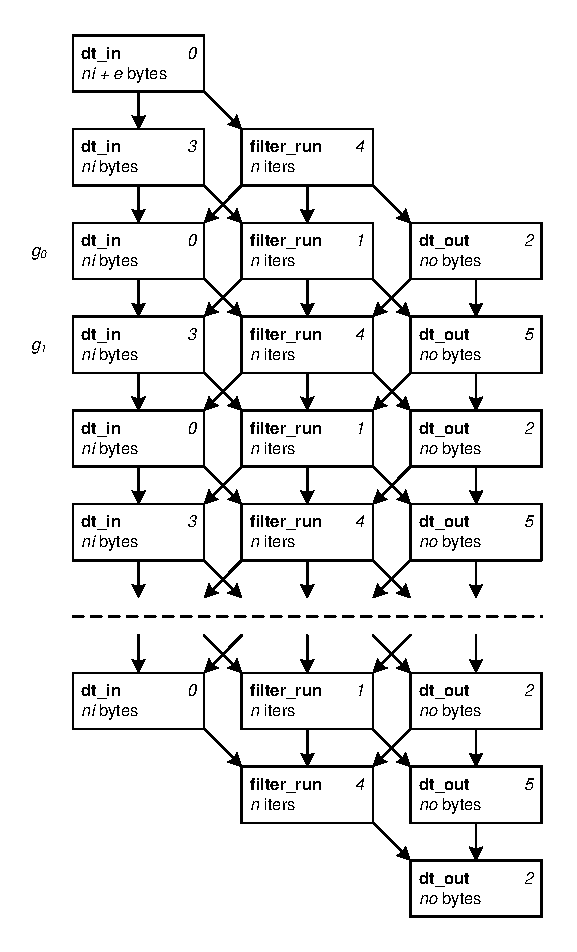
\includegraphics{figs/ext}
\end{center}
\caption[Sequence of commands to run a filter for a large number of iterations.]{Sequence of commands to run a filter for a large number of iterations. Command IDs are indicated in the upper right. Each row is issued as a different group.}
\label{fig:lib:ext}
\end{figure}

Provided that the input buffer is at least $2ni+e$ bytes and the output buffer is at least $2no$ bytes, the dependencies among the commands in the sequence ensure that:
\begin{itemize}
\item When a \textsf{dt\_in} command becomes active, there are at most $ni+e$ bytes of data in the input buffer, and thus enough space to transfer in an additional $ni$ bytes.
\item When a \textsf{dt\_out} command becomes active, there are at least $no$ bytes of data in the output buffer, and thus enough data to transfer out.
\item When a \textsf{filter\_run} command becomes active, there are at least $ni+e$ bytes of data in the input buffer and at most $no$ bytes of data in the output buffer. This is enough input data and output space to run the filter for $n$ iterations.
\end{itemize}

This sequence of commands effectively ``pipelines'' the basic operation from figure~\ref{fig:lib:run}. Double-buffering is accomplished when the data transfer commands in a group complete before the \textsf{filter\_run} does. In this case, the following \textsf{filter\_run} has no outstanding dependencies once the current \textsf{filter\_run} completes, and can become active immediately.

The user can keep the SPE continually supplied with work by initially issuing the first two groups, thereafter issuing the next group whenever a group completes. In this case, the SPE almost always has two groups of commands issued, with one group active and the other queued. In addition, with the exception of the first two and last two groups, the command parameters, IDs and dependencies in every other group are identical. This allows the user to initially set up two groups ($g_0$ and $g_1$ in figure~\ref{fig:lib:ext}) and repeatedly issue them for a majority of the execution. If executions are relatively long, the overhead of the first and last group, where no filter is being run, will be amortized effectively. Alternatively, the user can load another filter and run it during those gaps.

In practice, situations such as the above, where a static-rate filter is run for a large number of iterations and large amounts of input and output data are transferred, are very common. To avoid requiring the user to manually issue groups and deal with command completion callbacks in every such case, the library also provides extended operations that encapsulate this pattern. In an extended operation, the user provides the library with filter rates, the addresses of opposing buffers on other processors for data transfers, and the number of groups to run for; the library issues and responds to all commands internally and notifies the user when the entire operation is complete. Where one or both opposing buffers are located in memory, the library also handles the PPE side of data transfers internally. Extended operations greatly simplify setting up pipelines of any length where all filters in the pipeline have static rates.

\section{Library Implementation}

The library is implemented as three separate components: \emph{i}) runtime code for SPEs, \emph{ii}) basic runtime code for the PPE, and \emph{iii}) runtime code for the PPE that handles extended operations.

\subsection{PPE Implementation}

For each SPE, the library maintains a fixed table of command groups in memory. Each entry in the table represents a group and stores command data for commands in the group. When the user issues a group to an SPE, the library sends a mailbox message to the SPE to notify it of the entry in the table that contains the group and the LS address to copy command data to; the use of a fixed table is directly necessary to be able to pack all required fields into a single 32-bit mailbox message. After receiving the mailbox message, library code on the SPE initiates DMA to copy command data into local store.

When commands are completed by an SPE, library code on the SPE sends a bitmap of the command ID(s) to the PPE via the outbound mailbox. If the mailbox is full (the PPE has not had time to respond to the previous message), the bitmap is queued and sent when the mailbox is empty. The size of a mailbox message (32 bits) currently imposes a strict limit on the range of valid command IDs.

Library code on the PPE continually polls the outbound mailboxes of all SPEs in round-robin order for command completion messages. When a message is received, it is processed by the library, which eventually runs the user-registered callback. Interrupts were not used as each interrupt requires approximately 7 $\mu$s of kernel time to process. Although this may be negligible when only a single SPE is involved, it can become significant when multiple SPEs are all generating interrupts. In general, it is the author's opinion that the Cell architecture's focus on directly using SPEs to run small pieces of application code is not suited for the additional system overhead of interrupts.

One major drawback of the continuous polling approach is that it severely constrains any other work that the PPE is able to perform unless the user is willing to call the library function that performs polling at regular intervals. This is not a problem when the PPE is used solely as a control processor; most control computations are in response to command completion messages from SPEs and can be done in the callback.

The sequence of events that occurs on the PPE and an SPE between the time the user issues a group of commands and the user being notified of the completion of a command in the group via callback is illustrated in figure~\ref{fig:lib:control}. In actuality, because \emph{i}) each SPE is issued multiple commands and \emph{ii}) the PPE is controlling multiple SPEs, there will typically be many different copies of this sequence interleaved within each other, for both the same and different SPEs.

\begin{figure}[!htb]
\begin{center}
\begin{tabular}{rp{2.5in}p{2.5in}}
& \emph{PPE} & \emph{SPE} \\
\cline{2-3}
& Continually polls for command completion messages from SPEs. & Continually polls for mailbox messages while running active commands. \\
\cline{2-3}
\textsf{(1)} & \emph{User creates new group and adds commands.} Command data is written to entry in groups table. & \\
& \emph{User issues group.} Sends mailbox message to SPE. & \\
& & Receives and unpacks mailbox message. Copies command data (using DMA) from table entry to local store at specified LS address. \\
& & After copying command data, adds new commands to dependency graph. \\
& & \multicolumn{1}{c}{$\cdots$} \\
& & When command(s) complete, writes bitmap of completed ID(s) to PPE. \\
& Receives command completion message and calls user-defined callback. & \\
& \emph{Inside callback, user sets up and issues new groups if desired.} Repeats from \textsf{(1)}. &
\end{tabular}
\end{center}
\caption[SPE control protocol.]{SPE control protocol. \emph{Italicized} text represents actions performed by user code. All other actions are performed by library code.}
\label{fig:lib:control}
\end{figure}

\subsection{SPE Implementation}

To execute multiple active commands concurrently on an SPE, the library implements what is effectively a simple co-operatively multitasked ``operating system''. Each type of command has an associated handler function that processes it, and all active commands on an SPE act as separate ``threads'' executing at separate points in their handler functions, using command data to store temporary state in lieu of a separate stack.

The library maintains a run list that contains all active commands in a circular linked list. At the top level, the library cycles through each command in the run list and calls its handler. Each handler performs a small amount of work, typically only part of the work the command specifies, and then returns to the run list to allow other commands to execute. For example, the handler for the \textsf{filter\_run} command runs the filter's work function for one iteration\footnote{To reduce library overhead for filters that have small work functions, the command actually accepts an additional parameter that specifies the number of iterations to run the work function in each cycle through the run list. Alternatively, the compiler can coarsen the work function directly.} and then returns, relinquishing control of the SPE to other commands; in total, the filter's work function is run once for every cycle through the run list. More complex command handlers, such as those for data transfer commands, implement a simple state machine, storing state variables in temporary space in command data. Commands that are queued (have dependencies that have not yet completed) are not placed on the run list and incur no overhead for commands that are running; this allows the user to queue commands according to convenience, with no penalty.

Commands that perform DMA, such as data transfer commands, can wait for DMA operations to complete after starting them. While waiting, the command is removed from the run list, incurring no overhead for commands that are still running. The SPE continues to run other active commands while the DMA is in progress, providing communication--computation concurrency. Once the DMA operation completes, the command is re-added to the run list and the state machine in the command handler will continue where it left off.

DMA completions and inbound mailbox messages are checked via polling instead of interrupts. The library framework allows this internal functionality to be implemented simply as other commands:
\begin{itemize}
\item A command that polls for DMA completions and wakes other commands. This command also sends queued command completion messages to the PPE.
\item A command that polls the inbound mailbox for new command groups from the PPE. This command must perform DMA to copy command data for the group into local store, and does so using the standard mechanism.
\end{itemize}

The library framework causes polling to be done once every cycle through the run list.

From an implementation perspective, the framework does not seem to add significant complexity. In particular, the handlers for data transfer commands have a number of states and consist of a large outer \textsf{switch} statement. However, data transfers, which involve waits, would be fairly complex in any case, and the only obfuscation forced by the framework is that the otherwise linear structure of the handler function is broken up by \textsf{switch} cases. The framework has the advantage of treating all commands uniformly -- any command handler can perform a data transfer -- and thus it allows the library to be easily extended with new commands.

From an efficiency perspective, the run list involves multiple branches that cannot be predicted and does add some overhead to an SPE's main task of running filter work functions. However, this is generally a small fraction of the time spent in even slightly computation-intensive work functions. The run list framework is also not fair in scheduling multiple \textsf{filter\_run} commands: instead of sharing the SPE equally, they are given time proportional to the time spent in a single iteration of their work functions. However, even a single active \textsf{filter\_run} command makes full use of an SPE, and there is commonly only a single running filter (in addition to data transfer commands).

The library completely avoids interrupts, and consequently relies on co-operative multitasking. This was done for a number of reasons. Foremost, the granularity of a filter work function, which typically performs a small amount of work, provides a natural unit of time for switching between commands. SPEs have no timer interrupt; regardless, no timer interrupt could provide the granularity required: a work function of a typical filter might take tens of microseconds to run. In addition, the large number of registers on SPEs makes register saving and restoring time-consuming if interrupts were to be used for DMA completions and inbound mailbox messages. The current framework also avoids any possibility of race conditions when implementing data transfer commands that access buffers: when a data transfer command handler is executing, all filters are between work function iterations and it is the only code accessing the buffer's head and tail pointers.

Since polling is done only at one specific point in the run list, additional latency is introduced into commands that perform DMA. However, this has no effect as long as the user can overlap data transfer commands with computation.
 
Library code occupies approximately the first 16 KB of local store. The remainder is available for use by filter code, filter state, buffers, and the stack.

\subsection{Data Transfer Implementation}

Data transfer between two buffers on different processors involves additional synchronization between the processors. In particular, the source processor communicates to the destination SPE (SPE to memory data transfer will be discussed later later) \emph{i}) that data is available in the source buffer and \emph{ii}) the value of the source buffer's head pointer, so the destination buffer knows where to copy data from. The interaction between a pair of corresponding data transfer commands is given in figure~\ref{fig:lib:dt}:

\begin{figure}[!htb]
\begin{center}
\begin{tabular}{p{2.5in}p{2.5in}}
\emph{Source} & \emph{Destination} \\
\hline
Writes head pointer (using DMA) to destination buffer's control block. & Polls for head pointer from source processor. \\
Polls for acknowledgement from destination SPE. & \\
& After receiving head pointer, starts DMA for actual data. \\
& After copying all data, writes acknowledgement to source buffer's control block. \\
After receiving acknowledgement, completes. & After write completes, completes.
\end{tabular}
\end{center}
\caption{SPE--SPE data transfer protocol.}
\label{fig:lib:dt}
\end{figure}

The actual copying of data is done in a ``pull'' manner by the destination SPE. The entire transfer may require more than one DMA operation when the total transfer size is larger than Cell's maximum 16 KB DMA size, or when either buffer wraps around. After starting a single DMA operation, the destination SPE waits for it to complete before starting the next (during this time, the command is removed from the run list and incurs no overhead).

Polling on both processors is done by checking the control block in the command handler and, if not successful, immediately returning to the run list. The next poll occurs when the command handler is run again the next time through the run list.

Transfers where the source buffer is located in memory (and thus handled by the PPE) differ slightly from the protocol presented above. The PPE can use the completion of the data transfer command on the destination SPE as the acknowledgement.

Transfers where the destination buffer is located in memory require separate handling. Although the PPE can start DMA operations from SPE local store, PPE-initiated DMA is less efficient and having PPE code handle transfers places an additional load on the PPE, which must service all SPEs. Instead, transfers to memory are performed in a ``push'' manner that is approximately the reverse of the protocol described above. The PPE uses the completion of the data transfer command on the source SPE as the acknowledgement; in this manner, polling other than for command completion messages is completely avoided on the PPE and multiple transfers to/from memory place no extra overhead on the PPE.

A single active data transfer command on an SPE does not make full use of the MFC, since it starts a single DMA operation and waits for it to complete before starting another. However, this is offset by two considerations: \emph{i}) there should typically be at least two active data transfer commands, one for the input and one for the output buffers and \emph{ii}) when double-buffering is done via the dependency graph, the slight increase in data transfer latency should have no effect.

For double-buffering to be successful, a \textsf{filter\_run} command that is active concurrently with data transfer commands must return to the run list enough times for the data transfer commands to be able to run completely. As a consequence, \textsf{filter\_run} commands should specify at least three or four iterations. In practice, most filter work functions produce and consume relatively small amounts of data per iteration, and this can be easily met even with relatively small buffer sizes.

\subsubsection{Unaligned Data Transfers}

Data transfers that do not begin on a quadword boundary\footnote{Where the head pointer of the source buffer and the tail pointer of the destination buffer are not aligned on a quadword.} require special handling, since the Cell architecture requires DMA operations of quadword size or larger to be quadword-aligned. It is not safe to DMA the entire quadword that contains the source buffer's head pointer directly into the destination buffer, since this overwrites data before the end of the destination buffer with data from before the front of the source buffer, which may be invalid (figure~\ref{fig:lib:dtua}a). Treating the unaligned portion of this quadword as a series of 1-, 2-, 4-, and 8-byte DMA operations (figure~\ref{fig:lib:dtua}b) produces a large amount of DMA overhead and is a poor use of Cell's communication network.

\begin{figure}[!htb]
\begin{center}
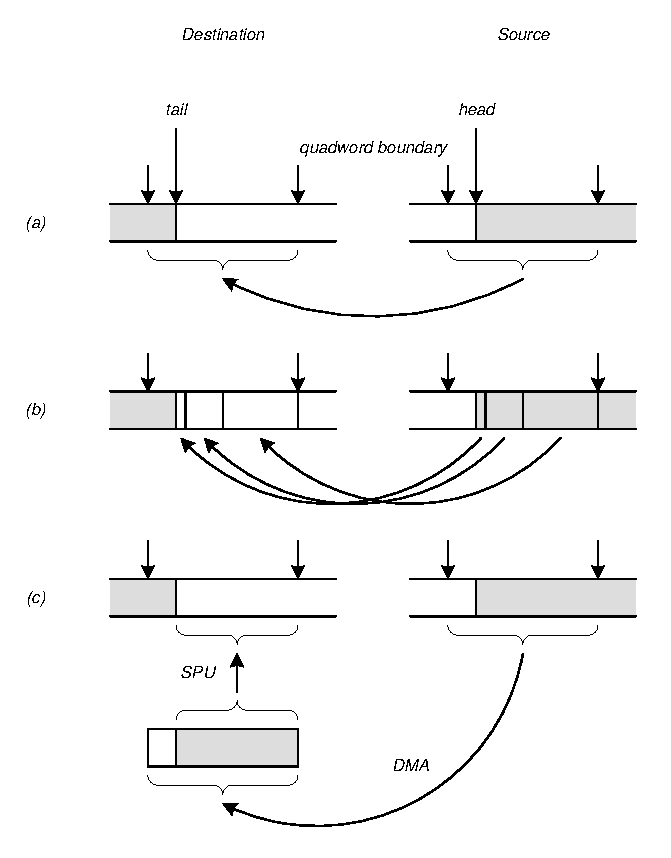
\includegraphics{figs/dt}
\end{center}
\caption[Different ways of handling unaligned data transfers.]{Different ways of handling unaligned data transfers. (a) is incorrect, since it overwrites data in the destination buffer with invalid data from the source buffer. (b) is correct but involves many DMA operations, and is less efficient. (c) is the actual method implemented.}
\label{fig:lib:dtua}
\end{figure}

Instead, the destination SPE DMAs the quadword from the source buffer into the destination buffer's control block, instead of directly into the buffer. When the DMA completes, the destination SPE writes only the valid portion of quadword into the destination buffer.\footnote{This is actually a read-modify-write operation, but it is done by the SPU, not the MFC.} This is illustrated in figure~\ref{fig:lib:dtua}c. The library uses intrinsics to avoid an expensive \textsf{for} loop. For transfers to a destination buffer located in memory, the source SPE DMAs the quadword to the destination buffer's control block and the PPE writes the valid portion of the quadword into the destination buffer using VMX intrinsics after the source command completes.

\section{Mapping StreamIt Patterns to the Runtime Library}\label{ch:use}

There are a number of common execution patterns that can be used to run a StreamIt program (see section~\ref{ch:bg:str:exec}). To illustrate how these patterns can be mapped to the runtime library for Cell, we will refer to the FFT StreamIt benchmark as a concrete example. This program performs a 256-element fast Fourier transform. The program's stream graph (figure~\ref{fig:use:fftgraph}) consists of a single pipeline of 15 filters. Every filter in the pipeline is stateless (and hence data-parallel) and does not peek. A single complete execution of the stream graph processes a single set of 256 input elements (512 floats), producing the same number of output elements.

\begin{figure}[!htb]
\begin{center}
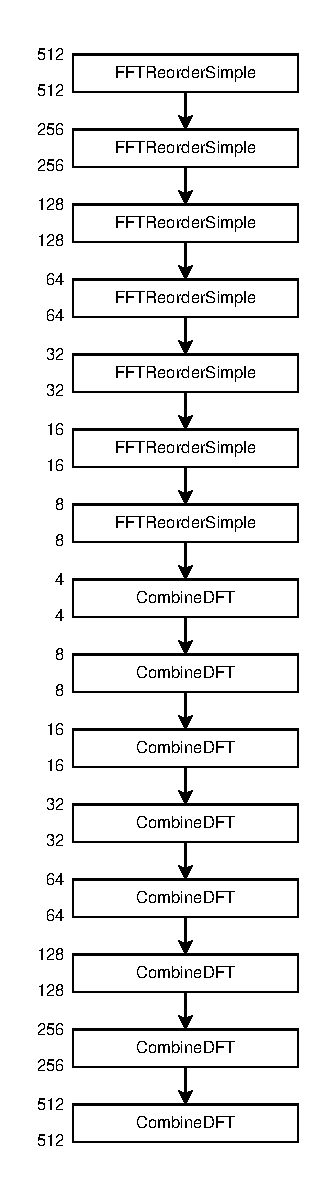
\includegraphics{figs/fftgraph}
\end{center}
\caption[Stream graph for 256-element FFT.]{Stream graph for 256-element FFT. A single execution of the stream graph pops and pushes 512 floats, since each element is a complex number whose components are interleaved on tapes.}
\label{fig:use:fftgraph}
\end{figure}

Data-parallel filters are the simplest to map to the library. The entire FFT pipeline can be fused into a single data-parallel filter that pops and pushes 512 floats per work function iteration. The fused filter can be data-parallelized over many SPEs: pseudocode to do this is illustrated in figure~\ref{fig:use:dp}. The \textsf{ext\_ppu\_spu\_ppu\_ex} library function starts an extended operation that loads the filter, allocates its buffers, and runs it for a large number of iterations.\footnote{The user still specifies all major parameters -- for example, the addresses to allocate buffers at and how many iterations each \textsf{filter\_run} command runs for.} The line containing \textsf{spulib\_poll\_while} synchronizes all SPEs; it returns only when all SPEs have finished and the callback has been run for each SPE.

\begin{figure}[!htb]
\begin{center}
\begin{tabular}{ll}
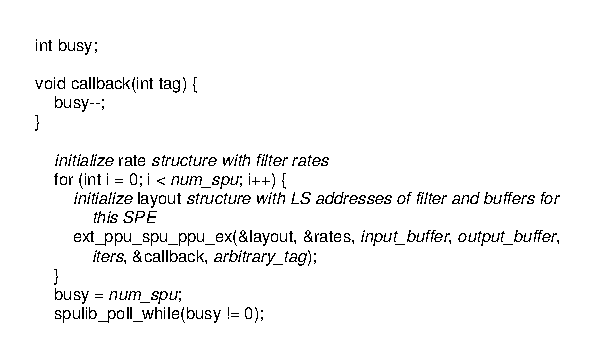
\includegraphics{figs/dpcode} & 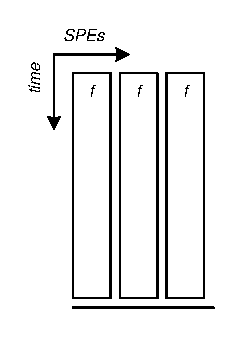
\includegraphics{figs/dp}
\end{tabular}
\end{center}
\caption[Pseudocode for running a data-parallel filter.]{Pseudocode for running a data-parallel filter. The figure on the right represents the state of each SPE as time passes. The horizontal line indicates synchronization by the PPE.}
\label{fig:use:dp}
\end{figure}

Course-grained software pipelining~\cite{asplos06} can be implemented similarly. Typically, the user will have assigned each filter in the steady state to an SPE and allocated and populated a buffer in memory for each channel. Pseudocode to execute a single iteration of the steady state is illustrated in figure~\ref{fig:use:swpipe}. Again, the line containing \textsf{spulib\_poll\_while} synchronizes all SPEs; this is necessary to ensure that sufficient input data has been produced for every filter in the next steady state iteration. For efficiency, the steady state should be sufficiently coarsened to amortize the overhead while SPEs are switching between filters and thus not performing any computation.

\begin{figure}[!htb]
\begin{center}
\begin{tabular}{ll}
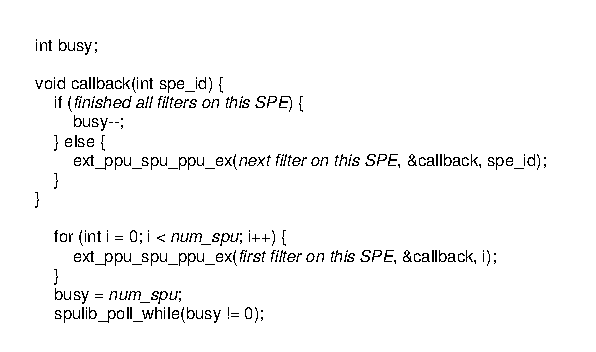
\includegraphics{figs/swpipecode} & 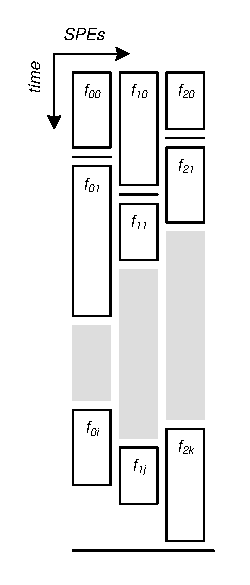
\includegraphics{figs/swpipe}
\end{tabular}
\end{center}
\caption[Pseudocode for running a course-grained software pipeline.]{Pseudocode for running a course-grained software pipeline. The figure on the right represents the state of each SPE as time passes. Horizontal lines indicate synchronization by the PPE.}
\label{fig:use:swpipe}
\end{figure}

Both patterns presented so far involve no direct SPE--SPE communication. An alternative implementation for FFT partially fuses the 15 filters in the StreamIt pipeline into a number of library filters, which are simultaneously run on different SPEs (figure~\ref{fig:use:spepipe}). These SPEs can transfer data between local stores directly, taking advantage of Cell's on-chip communication network and avoiding the extra latency to memory, as well as preventing memory from possibly becoming a bottleneck. Pseudocode to do this is illustrated in figure~\ref{fig:use:spepipecode}.

\begin{figure}[!htb]
\begin{center}
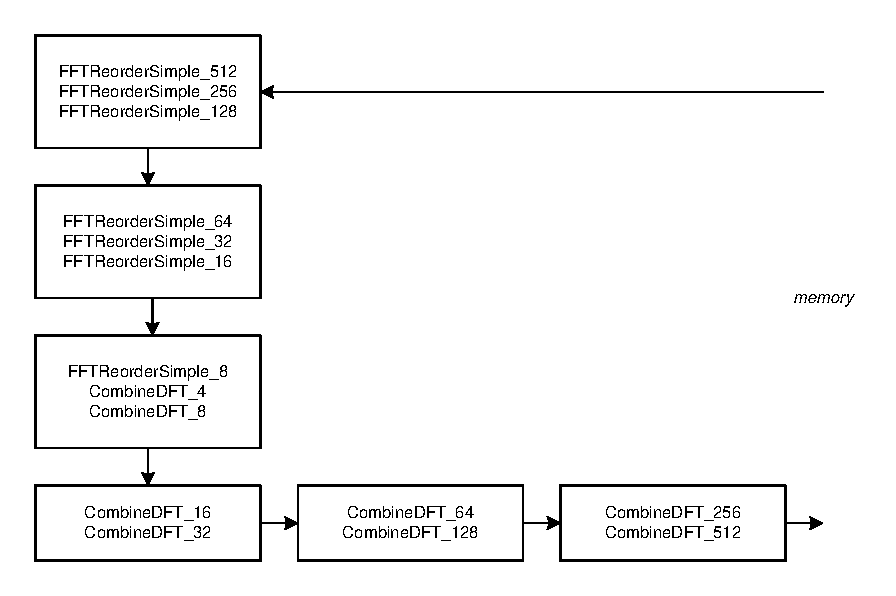
\includegraphics{figs/spepipe}
\end{center}
\caption{Pipelining FFT over six SPEs.}
\label{fig:use:spepipe}
\end{figure}

\begin{figure}[!htb]
\begin{center}
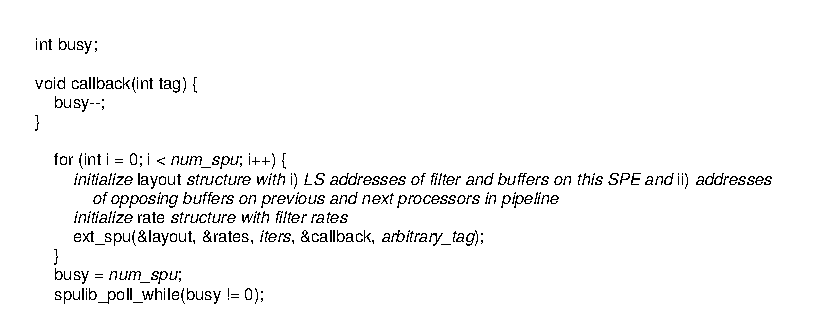
\includegraphics{figs/spepipecode}
\end{center}
\caption{Pseudocode for setting up an SPE--SPE pipeline.}
\label{fig:use:spepipecode}
\end{figure}

More complex scheduling choices require the user to provide more complex callback functions. For example, the communication overhead of loading a new filter onto an SPE can be hidden if the load is performed while the old filter is still running its last iterations.

The library allows the user to treat filters as individual schedulable entities, instead of having to consider complex lower-level operations. The pseudocode in figure~\ref{fig:use:dp} can be compared to the SPE code required to execute the same pattern (a single fused data-parallel filter) without using the library, illustrated in figure~\ref{fig:use:handcode}.

\begin{figure}[!htb]
\begin{center}
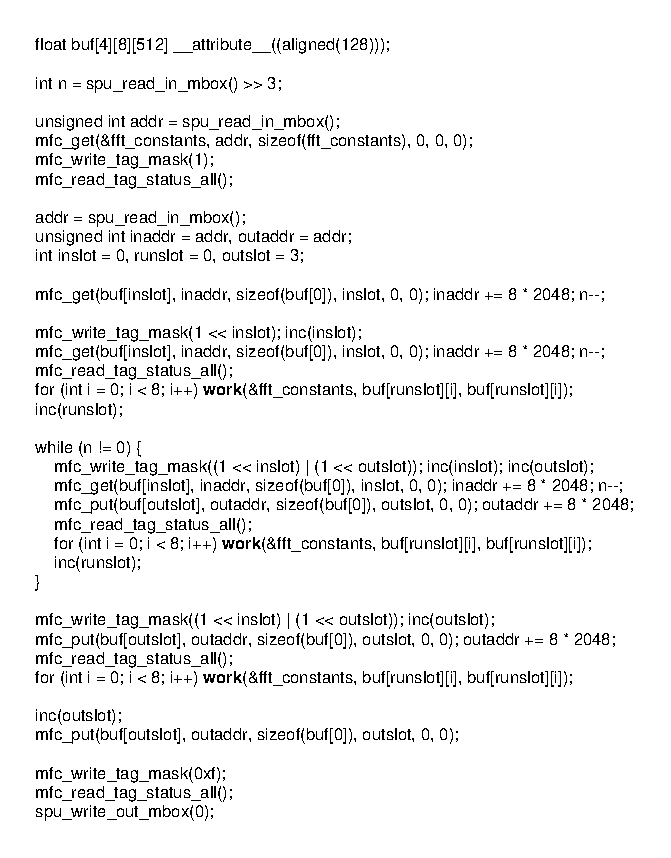
\includegraphics{figs/handcode}
\end{center}
\caption[SPE code for hand-coded implementation of data-parallel fused FFT.]{SPE code for hand-coded implementation of data-parallel fused FFT. The three bolded calls to \textsf{work} actually run the fused work function; the rest of the code performs double-buffered data transfers.}
\label{fig:use:handcode}
\end{figure}

This code is not overly complex, and will always be more efficient than using the library. However, this code is also specific to the filter and the execution pattern. The fused filter in FFT does not peek, and conveniently produces and consumes amounts of data that are compatible with Cell's DMA alignment requirements. The code would have to be significantly changed if a filter with slightly different rates were substituted. If multiple filters need to be run on an SPE, the code would then acquire additional logic to switch between filters. To run filters in an SPE--SPE pipeline, additional code would be needed to synchronize between SPEs. Using the library, the user does not need to deal with any of this.

\section{Splitters and Joiners}

In general, the type of fine-grained data reorganization performed by round-robin splitters and joiners cannot be directly implemented using Cell's DMA mechanism, which has strict alignment requirements. However, since the library supports filters with multiple input and/or output tapes, a compiler can simply define separate filters for each splitter and joiner. A compiler can also fuse a splitter or joiner with the upstream or downstream filter, respectively; the resulting filter has a much lower communication--computation ratio than an independent splitter or joiner.

The user can ignore duplicate splitters as long as the output of the upstream filter is buffered into memory. Because multiple PPE buffers can refer to the same data region, no duplication of data in memory is necessary. However, if the filters downstream of the splitter run on different SPEs, the same data must be copied to the local store of each SPE.

\section{Runtime Checks}

The library implements a number of runtime checks that can be enabled or disabled at compile time. When enabled, the library validates buffers accesses to ensure that they contain sufficient data/space, and performs additional checks to ensure that issued commands are consistent. While this cannot identify all bugs in a schedule or filter work function, it has nonetheless been very useful during the development of the library, the dynamic scheduler, and test programs; it has often exposed bugs that would otherwise only appear as a hung program or incorrect output.

\section{Filter Code Limitations}

To the author's knowledge, in general GCC is unable to easily generate filter code that contains no absolute loads or branches. As a result, currently code for all filters must permanently occupy space in SPE local store. This does not significantly affect most FFT implementations, since the program's work functions are quite small.

\section{Dynamic Scheduling Using the Runtime Library}\label{ch:ds}

The dynamic scheduler is implemented as a layer on top of the runtime library. Like the library, it is designed for but not specific to StreamIt: it can schedule any acyclic stream graph where all filters have static rates, subject to some additional limitations.\footnote{The dynamic scheduler places a maximum limit on the degree of any node in the stream graph.} A StreamIt program can be converted filter-by-filter into input to the dynamic scheduler, or a compiler can first perform high-level optimizations that modify the original stream graph.

We first discuss the advantages offered by a dynamic scheduling approach in section~\ref{ch:ds:bg} before discussing the interface and implementation of the actual scheduler in sections~\ref{ch:ds:ui} and \ref{ch:ds:imp}.

\section{Dynamic Scheduling vs. Static Scheduling}\label{ch:ds:bg}

For stream graphs that are ``well-behaved'', dynamic scheduling generally does not present any advantages over static scheduling. Dynamic scheduling inevitably involves additional communication and scheduling overhead due to extra filter loading and unloading, buffer management, and scheduling computation. When all filters in a program are data-parallel, a static scheduler can make full use of all SPEs by simply executing each filter in turn on all SPEs, with a sufficient coarsening of the steady state to amortize filter load/unload and SPE synchronization overhead. The optimal situation results when the compiler can fuse all filters into a single data-parallel filter; this produces the minimum possible communication.

Even when filters are stateful and thus cannot be data-parallelized, static software pipelining techniques~\cite{asplos06} can make full use of SPEs when the compiler has an accurate static work estimator and can divide filters in a steady state evenly across SPEs.\footnote{A single stateful filter with a heavily imbalanced work function creates a bottleneck, but dynamic schedulers are also faced with this problem.} In addition, no ``unpredictable'' cache misses or lengthy communication delays that can skew a static work estimate are possible on the Cell architecture.

Dynamic scheduling becomes beneficial when filters are not ``well-behaved'': when it is difficult to statically balance load across SPEs, difficult to estimate the amount of work done by filter work functions, or work functions perform widely varying amounts of work through the execution of the program. In these situations, dynamic scheduling may be able to deliver better load-balancing than static scheduling.

A dynamically scheduled program can be run on varying numbers of processors without requiring recompilation or the reanalysis that complex static schedulers would need to perform, and is also tolerant of changes in the availability of processors while the program is running. In addition, for stream graphs that contain filters with dynamic rates, it may not be possible to statically predict how many times filters will be run, and the balance of work in the stream graph may change as the program is run. In this case, only dynamic scheduling is able to shift workload to different portions of the stream graph as needed.\footnote{However, the current dynamic scheduler implementation does not support dynamic rates.}

\section{User Interface}\label{ch:ds:ui}

The user provides as input to the dynamic scheduler a complete description of the stream graph, specifying filters and the channels that connect them. Rates for all filters must be specified. Duplicate splitters can be handled by setting parameters of channels; round-robin splitters and joiners must be defined as separate filters.

\section{Implementation}\label{ch:ds:imp}

The Cell architecture's communication network provides very high memory bandwidth. The design of the dynamic scheduler assumes that memory will never be a bottleneck (a hypothesis that was confirmed by experiments; see chapter~\ref{ch:perf}), and the dynamic scheduler buffers all output produced on SPEs to memory. The scheduler performs dynamic course-grained software pipelining on the stream graph; if sufficient data can be buffered in all channels at all times, pipeline stalls can be avoided and all SPEs can be fully utilized. While SPE--SPE communication is more efficient than SPE--memory communication, SPE local store is generally too limited to store the buffering needed for software pipelining, and thus the scheduler never executes SPE--SPE pipelines; this avoids having to deal with work imbalances between pairs of adjacent filters. At any time, any two SPEs will typically be operating on data from widely separated iterations of the program.

At startup, the dynamic scheduler allocates a large\footnote{1 MB in the current implementation, but this can be adjusted.} buffer in memory for each channel; this is used to buffer the output of the upstream filter to provide input for the downstream filter. At any time, for any specific filter, the amount of data available in its input channels and amount of space available in its output channels, along with its rates, determines the maximum number of iterations that the filter can be run for.

The scheduler selects filters to run on SPEs based on a metric computed from the maximum number of iterations and certain filter properties (see below). When a filter is selected to run on an SPE, it is scheduled for a limited but fairly large number of iterations in order to amortize the cost of loading it. Filters run for their entire allotment of iterations; however, allotments are kept small to allow the scheduler to quickly schedule another filter if necessary in response to the changing state in the stream graph.

A replacement filter for an SPE is selected when the current filter scheduled on the SPE has almost finished running for all of its allotted iterations. While the current filter is still running, the scheduler issues additional commands to load the new filter, allocate its buffers, and transfer data into its input buffers from memory; this communication is overlapped with the computation done by the current filter. When the replacement filter is the same as the current filter, this additional work can be avoided. Finally, the first command to run the new filter is queued after the last command to run the current filter. When the replacement filter is selected early enough, it will be set up on the SPE before the current filter finishes running, ensuring that it can start running as soon as the current filter finishes. When the current filter has completed all of its allotted iterations, it is unloaded and can then be scheduled on another SPE.

The dynamic scheduler can run multiple instances of data-parallel filters on multiple SPEs at the same time. A data-parallel filter is still selected by the same metric as other filters; it will only be run on more than one SPE at once if it is significantly better than other filters.

The current metric implemented is very simple: it prioritizes filters based on the amount of data the state of their input and output channels allow them to consume and produce, respectively. However, the filter that is currently running on an SPE is prioritized when considered for scheduling on the same SPE; this effectively causes filters to be run for as long as possible on an SPE, with no load overhead, while no other filters are significantly better. Other more complex metrics can be easily substituted.

When the dynamic scheduler encounters a pipeline, the filter selection metric quickly causes all filters in the pipeline to be run sufficiently to generate some data in every channel buffer. Thereafter, the sequence of filter executions selected by the scheduler appears to perform software pipelining, although without a recognizable steady state.

\chapter{Performance}\label{ch:perf}

Performance evaluation for the runtime library and dynamic scheduler was conducted by comparing different implementations of the FFT StreamIt program described in chapter~\ref{ch:use}. Six different implementations were tested:
\begin{enumerate}
\item FFT pipeline fused to single filter. All other infrastructure hand-coded and optimized.
\item Single fused filter, executed data-parallel using the library.
\item Full FFT pipeline, executed using dynamic scheduler, filters not specified as data-parallel.
\item Full FFT pipeline, executed using dynamic scheduler, filters specified as data-parallel.
\item Single fused filter, executed using dynamic scheduler, specified as data-parallel.
\item FFT pipeline partially fused to six filters, pipelined across six SPEs with direct SPE--SPE communication.
\end{enumerate}

The resulting programs were executed on PlayStation 3 hardware, which only provides six usable SPEs. During each execution, a program processed 20,000 iterations of data (approximately 20 MB). Each program iteration performs 16,384 floating point operations, for a total of 327 MFLOP. Runtimes for one and six SPEs are given in figure~\ref{fig:perf:fft} (file I/O time is excluded).

\begin{figure}[!htb]
\begin{center}
\begin{tabular}{|r|r|r|r|r|r|r|r|}
\hline
& \multicolumn{3}{|c|}{1 SPE} & \multicolumn{4}{|c|}{6 SPEs} \\
\cline{2-8}
& Time & Run \% & Work \% & Time & Run \% & Work \% & Speedup \\
\hline
\textsf{1} & 396.1 & \multicolumn{2}{|c|}{} & 66.6 & \multicolumn{2}{|c|}{} & 5.95 \\
\hline
\textsf{2} & 401.0 & 100.0 & 99.2 & 67.2 & 99.7 & 98.8 & 5.97 \\
\hline
\textsf{3} & 545.9 & 99.6 & 91.8 & 91.7 & 99.2 & 91.4 & 5.95 \\
\hline
\textsf{4} & \multicolumn{3}{|c|}{} & 91.9 & 99.0 & 91.2 & \\
\hline
\textsf{5} & 401.0 & 100.0 & 99.2 & 67.6 & 99.7 & 98.8 & 5.93 \\
\hline
\textsf{6} & \multicolumn{3}{|c|}{} & 86.2 & 95.9 & 92.2 & \\
\hline
\end{tabular}
\end{center}
\caption{Performance of different implementations of FFT.}
\label{fig:perf:fft}
\end{figure}

The \emph{Time} column gives the total time SPEs ran for, excluding one-time initialization done at the start of the program. Times are in milliseconds. For the five implementations that used the library, additional statistics maintained by the library are given. The \emph{Run \%} column gives the percentage of total time the SPE had an active \textsf{filter\_run} command. The remainder is overhead due to either \emph{i}) durations when SPEs do not have useful work to do (such as when waiting for filters to be loaded) or \emph{ii}) inadequate double-buffering of input or output data. In both cases, the scheduler (or the nature of the program) creates insufficient communication--computation concurrency. The \emph{Work \%} column gives the percentage of total time actually spent in the work function. The remainder represents the total overhead added by the library or caused by the scheduling algorithm. The large number of iterations tests ran for smoothes out any one-time execution startup overhead. For the tests involving six SPEs, the percentages given are for the SPE that reported the greatest work percentage. The \emph{Speedup} column gives the speedup relative to the same implementation on one SPE, where applicable.

Not surprisingly, hand-coded implementation \textsf{(1)} demonstrates almost perfect linear speedup on six SPEs.

Comparing results for implementation \textsf{(2)} to \textsf{(1)}, the overhead added by the library is around 1\%. Run \% is high, although not exactly 100\% due to the overhead of starting a long-term filter execution (loading the filter and allocating and attaching buffers). For both \textsf{(1)} and \textsf{(2)}, statistics for all SPEs were almost identical; this is not surprising given that the fused filter's work function performs a constant amount of work per iteration.

For implementations \textsf{(3)} and \textsf{(4)}, which involved the full pipeline on the dynamic scheduler, all six SPEs reported similar statistics (both absolute and percentage), indicating that the scheduler can make equal use of all available SPEs. Compared to implementation \textsf{(2)}, these implementations are 36\% slower. However, a large part of this can be accounted for by the observation that the total time spent in work functions in these implementations is 26\% greater. This is due to slightly more efficient code that is generated for the fused filter.

Run \% is slightly lower than in implementation \textsf{(2)}, but still fairly close to 100\%, and speedup on six SPEs is still almost perfectly linear; this indicates that the dynamic scheduler has no difficulties keeping all SPEs supplied with work. Moreover, it validates the critical assumption made in the design of the dynamic scheduler: the Cell architecture's memory bandwidth is indeed sufficient to perform all buffering to memory, avoiding SPE--SPE communication entirely. However, the lower Work \% indicates that the additional commands issued to SPEs by the dynamic scheduler to constantly switch filters do create a noticeable overhead: 8.6\% of total time, compared to 1.2\% for the data-parallel, fused, statically-scheduled implementation.

Not surprisingly, the almost identical results for implementations \textsf{(5)} and \textsf{(2)} indicate that the dynamic scheduler can execute a single fused data-parallel filter just as efficiently as a static schedule.

Implementation \textsf{(6)}, which pipelines multiple filters across SPEs, produces different results than the others. In this case, a single filter/SPE in the middle of the pipeline is a significant bottleneck; this is not surprising, since 15 filters were fused into six. Although total runtime is significantly worse than the hand-coded or fused data-parallel implementations, no SPE except for the bottleneck was fully utilized: two other SPEs had Work \% around 60\%. In general, this illustrates the difficulty of performing SPE--SPE pipelining. Although this implementation keeps communication on-chip (except for input and output to the pipeline), work imbalances make it difficult to fully utilize all SPEs.

\chapter{Conclusion}

    We present a methodology for the detection, analysis, combination, and
optimization of linear state-space filters in DSP applications.
This work is automatized in the compiler of a high-level
programming language, StreamIt, designed for streaming
applications. This frees the programmer from the burden of writing
low-level optimized code that requires expert DSP analysis.
Instead, the programmer can focus on the top-level design of a DSP
application and write modular code in a structured setting.

    Due to the infinite number of possible state-space transforms,
the optimizations discussed are not necessarily ideal.
Additionally, parts of DSP applications are non-linear and cannot
be analyzed in the state-space domain. Therefore, the work
presented in this thesis does not fully optimize some portions of
DSP applications, and does not apply towards other portions.
However, it does represent an additional step towards the goal of
a full analysis and optimization of any application. We outline
some of the future steps that can be taken, both to improve on the
work in this thesis and to expand it to other types of
domain-specific analyses and optimizations.
\begin{itemize}

\item As mentioned in Chapter 4, minimally parameterize a system,
then uses multiple execution stages.

\item Use a balanced representation \cite{Moore} to quantify the
relative impact of each state of a filter on its execution. Then
the states that have impact values below a certain threshold can
be removed, resulting in only a small change in the filter's
execution.

\item Formulate loops in traditional programming languages as
state-space filters, and use state-space work developed in this
thesis to detect their induction variables and optimize their
execution.

\item Create a cost function metric,
$f(\mathbf{A},\mathbf{B},\mathbf{C},\mathbf{D})$, that balances
the traditional program analysis metrics (throughput, power
consumption, memory allocation, etc.) in any manner desired. Then
find a general way to minimize this cost function over all
possible state-space transformations $\mathbf{T}$.

\item Formulate a methodology to deal with filters whose outputs
are a linear combination of their inputs but a non-linear
combination of their state variables.

\item Use a `black box' method to find the appropriate
representation of a filter. In this approach the filter is given
inputs and the output data is collected. The input/output
relations are used to formulate an appropriate state-space model
that may not exactly represent the filter, but does so within a
tolerable error margin (see \cite{Schutter}).
\end{itemize}

\appendix
\chapter{Benchmark Source Code}

    This is the StreamIt source code for the applications used in
the Results chapter. All code is copyrighted to MIT.

\vspace{50pt}

Library Files (for use with FMRadio, FIR Program, and Channel
Vocoder)
\begin{scriptsize}
\begin{verbatim}

/**
 * Simple sink that just prints the data that is fed to it.
 **/
float->void filter FloatPrinter {
  work pop 1 {
    println(pop());
  }
}


/**
 * Simple FIR low pass filter with gain=g, wc=cutoffFreq(in radians) and N samples.
 * Eg:
 *                 ^ H(e^jw)
 *                 |
 *          ---------------
 *          |      |      |
 *          |      |      |
 *    <-------------------------> w
 *         -wc            wc
 *
 * This implementation is a FIR filter is a rectangularly windowed sinc function
 * (eg sin(x)/x), which is the optimal FIR low pass filter in
 * mean square error terms.
 *
 * Specifically, h[n] has N samples from n=0 to (N-1)
 * such that h[n] = sin(cutoffFreq*pi*(n-N/2))/(pi*(n-N/2)).
 * and the field h holds h[-n].
 */
float->float filter LowPassFilter(float g, float cutoffFreq, int
N) {
  float[N] h;

  /* since the impulse response is symmetric, I don't worry about reversing h[n]. */
  init {
    int OFFSET = N/2;
    for (int i=0; i<N; i++) {
      int idx = i + 1;
      // generate real part
      if (idx == OFFSET)
    /* take care of div by 0 error (lim x->oo of sin(x)/x actually equals 1)*/
    h[i] = g * cutoffFreq / pi;
      else
    h[i] = g * sin(cutoffFreq * (idx-OFFSET)) / (pi*(idx-OFFSET));
    }
  }

  /* implement the FIR filtering operation as the convolution sum. */
  work peek N pop 1 push 1 {
    float sum = 0;
    for (int i=0; i<N; i++) {
      sum += h[i]*peek(i);
    }
    push(sum);
    pop();
  }
}


/**
 * Simple FIR high pass filter with gain=g, stopband ws(in radians) and N samples.
 *
 * Eg
 *                 ^ H(e^jw)
 *                 |
 *     --------    |    -------
 *     |      |    |    |     |
 *     |      |    |    |     |
 *    <-------------------------> w
 *                   pi-wc pi pi+wc
 *
 *
 * This implementation is a FIR filter is a rectangularly windowed sinc function
 * (eg sin(x)/x) multiplied by e^(j*pi*n)=(-1)^n, which is the optimal FIR high pass filter in
 * mean square error terms.
 *
 * Specifically, h[n] has N samples from n=0 to (N-1)
 * such that h[n] = (-1)^(n-N/2) * sin(cutoffFreq*pi*(n-N/2))/(pi*(n-N/2)).
 * where cutoffFreq is pi-ws
 * and the field h holds h[-n].
 */
float->float filter HighPassFilter(float g, float ws, int N) {
  float[N] h;

  /* since the impulse response is symmetric, I don't worry about reversing h[n]. */
  init {
    int OFFSET = N/2;
    float cutoffFreq = pi - ws;
    for (int i=0; i<N; i++) {
      int idx = i + 1;
      /* flip signs every other sample (done this way so that it gets array destroyed) */
      int sign = ((i%2) == 0) ? 1 : -1;
      // generate real part
      if (idx == OFFSET)
    /* take care of div by 0 error (lim x->oo of sin(x)/x actually equals 1)*/
    h[i] = sign * g * cutoffFreq / pi;
      else
    h[i] = sign * g * sin(cutoffFreq * (idx-OFFSET)) / (pi*(idx-OFFSET));
    }

  }

  /* implement the FIR filtering operation as the convolution sum. */
  work peek N pop 1 push 1 {
    float sum = 0;
    for (int i=0; i<N; i++) {
      sum += h[i]*peek(i);
    }
    push(sum);
    pop();
  }
}


/* This is a bandpass filter with the rather simple implementation
of
 * a low pass filter cascaded with a high pass filter. The relevant parameters
 * are: end of stopband=ws and end of passband=wp, such that 0<=ws<=wp<=pi
 * gain of passband and size of window for both filters. Note that the high
 * pass and low pass filters currently use a rectangular window.
 **/
float->float pipeline BandPassFilter(float gain, float ws, float
wp, int numSamples) {
  add LowPassFilter(1, wp, numSamples);
  add HighPassFilter(gain, ws, numSamples);
}


/**
 * This filter compresses the signal at its input by a factor M.
 * Eg it inputs M samples, and only outputs the first sample.
 **/
float->float filter Compressor(int M) {
  work peek M pop M push 1 {
    push(pop());
    for (int i=0; i<(M-1); i++) {
      pop();
    }
  }
}

\end{verbatim}
\end{scriptsize}


FM Radio
\begin{scriptsize}
\begin{verbatim}

/*
 * Software equalizer.  This version uses n+1 low-pass filters directly,
 * as opposed to n band-pass filters, each with two low-pass filters.
 * The important observation is that we have bands 1-2, 2-4, 4-8, ...
 * This means that we should run an LPF for each intermediate frequency,
 * rather than two per band.  Calculating this in StreamIt isn't that bad.
 * For a four-band equalizer:
 *
 *              |
 *             DUP
 *    +---------+---------+
 *    |         |         |
 *    |        DUP        |
 *    |    +----+----+    |
 *    |    |    |    |    |
 *   16    8    4    2    1
 *    |    |    |    |    |
 *    |  (dup)(dup)(dup)  |
 *    |    |    |    |    |
 *    |    +----+----+    |
 *    |       RR(2)       |
 *    |         |         |
 *    +---------+---------+
 *       WRR(1,2(n-1),1)
 *              |
 *            (a-b)
 *              |
 *            SUM(n)
 *              |
 *
 * It's straightforward to change the values of 1, 16, and n.  Coming out
 * of the EqualizerSplitJoin is 16 8 8 4 4 2 2 1; we can subtract and scale
 * these as appropriate to equalize.
 */


float->float filter FloatNAdder(int count) {

  work push 1 pop count {

    float sum = 0.0;

    for(int i=0; i<count; i++)
      sum += pop();

    push(sum);
  }
}


float->float filter FloatDiff() {

  work push 1 pop 2 {

    push(peek(0) - peek(1));
    pop();
    pop();
  }
}


float->float filter FloatDup() {

  work push 2 pop 1 {

    float val = pop();
    push(val);
    push(val);
  }
}


float->float pipeline EqualizerInnerPipeline(float rate, float
freq) {

  add FMLowPassFilter(rate,freq,64,0);
  add FloatDup();
}


float->float splitjoin EqualizerInnerSplitJoin(float rate, float
low, float high, int bands) {

  split duplicate();
  for(int i=0; i < bands-1; i++)
    add EqualizerInnerPipeline(rate,(float)exp((i+1)*(log(high)-log(low))/bands + log(low)));
  join roundrobin(2);
}


float->float splitjoin EqualizerSplitJoin(float rate, float low,
float high, int bands) {

  split duplicate();
  add FMLowPassFilter(rate,high,64,0);
  add EqualizerInnerSplitJoin(rate,low,high,bands);
  add FMLowPassFilter(rate,low,64,0);
  join roundrobin(1,(bands-1)*2,1);
}


float->float pipeline Equalizer(float rate) {

  int bands = 10;
  float low = 55;
  float high = 1760;

  add EqualizerSplitJoin(rate,low,high,bands);
  add FloatDiff();
  add FloatNAdder(bands);
}


float->float filter FMLowPassFilter(float sampleRate, float
cutFreq, int numTaps, int decimation) {

  float[numTaps] COEFF;     //all frequencies are in hz
  float tapTotal;

  init {
    float m = numTaps -1;
    //from Oppenheim and Schafer, m is the order of filter

    if(cutFreq == 0.0) {

      //Using a Hamming window for filter taps:
      tapTotal = 0;

      for(int i=0;i<numTaps;i++) {
    COEFF[i] = (float)(0.54 - 0.46*cos((2*pi)*(i/m)));
    tapTotal = tapTotal + COEFF[i];
      }

      //normalize all the taps to a sum of 1
      for(int i=0;i<numTaps;i++) {
    COEFF[i] = COEFF[i]/tapTotal;
      }
    }
    else{
    //ideal lowpass filter ==> Hamming window
    //has IR h[n] = sin(omega*n)/(n*pi)
    //reference: Oppenheim and Schafer

    float w = (2*pi) * cutFreq/sampleRate;

    for(int i=0;i<numTaps;i++) {
      //check for div by zero
      if(i-m/2 == 0)
    COEFF[i] = w/pi;
      else
    COEFF[i] = (float)(sin(w*(i-m/2)) / pi
                   / (i-m/2) * (0.54 - 0.46
                        * cos((2*pi)*(i/m))));
      }
    }
  }

  work push 1 pop decimation+1 peek numTaps {
    float sum = 0.0;
    for(int i=0; i<numTaps; i++) {
      sum += peek(i)*COEFF[i];
    }
    pop();
    for(int i=0; i<decimation; i++)
      pop();

    push(sum);

  }
}


float->float filter FMDemodulator(float sampRate, float max, float
bandwidth) {

  float mGain;

  init {
    mGain = max*(sampRate/(bandwidth*pi));
  }

  work push 1 pop 1 peek 2 {
    float temp = 0;
    //may have to switch to complex?
    temp = (float)(peek(0) * peek(1));
    //if using complex, use atan2
    temp = (float)(mGain * atan(temp));

    pop();
    push(temp);
  }
}


void->float filter FloatOneSource {

  float x;

  init {
    x = 0;
  }

  work push 1 pop 0 {
    push(x++);
  }
}


/*
 * Early attempt at an FM Radio... probably junk
 */

float->float pipeline FMRadioCore {

    // float samplingRate = 200000; //200khz sampling rate according to jeff at vanu
    float samplingRate = 250000000; // 250 MHz sampling rate much more sensible, though
    float cutoffFrequency = 108000000; //guess... doesn't FM freq max at 108 Mhz?
    int numberOfTaps = 64;
    float maxAmplitude = 27000;
    float bandwidth = 10000;
    //decimate 4 samples after outputting 1
    add FMLowPassFilter(samplingRate, cutoffFrequency, numberOfTaps, 4);
    add FMDemodulator(samplingRate, maxAmplitude, bandwidth);
    add Equalizer(samplingRate);
}


void->void pipeline FMRadio {

  add FloatOneSource();
  add FMRadioCore();
  add FloatPrinter();
}

\end{verbatim}
\end{scriptsize}


FIR Program
\begin{scriptsize}
\begin{verbatim}

/**
 * This streamit program contains a simple low pass filter
 * that filters the data from a source and funnels it directly
 * to a sink. This is more of a "kernel" type benchmark because
 * FIR filtering is widely used in actual DSP applications.
 **/

/**
 * Top level program.
 **/
void->void pipeline FIRProgram {
  add FloatSource();
  add LowPassFilter(1, pi/3, 256);
  add FloatPrinter();
}

/**
 * Simple float source -- puts out a ramp from
 * 0 to 15 over and over again. Note that it
 * generates its output data in its init function
 * and the oly work that occurs in the work function
 * is pushing the data on to the tape and doing some
 * buffer management.
 **/
void->float filter FloatSource {
  float[16] inputs;
  int idx;
  init {
    for(int i=0; i<16; i++) {
      inputs[i] = i;
    }
    idx = 0;
  }
  work push 1 {
    push(inputs[idx]);
    idx = (idx + 1) % 16;
  }
}

\end{verbatim}
\end{scriptsize}


Channel Vocoder
\begin{scriptsize}
\begin{verbatim}

/**
 * This is a channel vocoder as described in 6.555 Lab 2.
 * It's salient features are a filterbank each of which
 * contains a decimator after a bandpass filter.
 *
 * Sampling Rate is 8000 Hz.
 * First the signal is conditioned using a lowpass filter with
 * cutoff at 5000 Hz. Then the signal is "center clipped" which
 * basically means that very high and very low values are removed.
 *
 * Then, the signal is sent both to a pitch detector and to a
 * filter bank with 200 Hz wide windows (18 overall)
 *
 * Thus, each output is the combination of 18 band envelope values
 * from the filter bank and a single pitch detector value. This
 * value is either the pitch if the sound was voiced or 0 if the
 * sound was unvoiced.
 **/
void->void pipeline ChannelVocoder {
  add DataSource();
  // low pass filter to filter out high freq noise
  add LowPassFilter(1, (2*pi*5000)/8000, 64);
  add MainSplitjoin();
  add FloatPrinter();
}

/** This class is just a wrapper so that we don't have anonymous
inner classes. **/ float->float splitjoin MainSplitjoin {
  int PITCH_WINDOW = 100; // the number of samples to base the pitch detection on
  int DECIMATION   = 50; // decimation factor
  int NUM_FILTERS  = 4; //18;

  split duplicate;
  add PitchDetector(PITCH_WINDOW, DECIMATION);
  add VocoderFilterBank(NUM_FILTERS, DECIMATION);
  join roundrobin(1,4); // can't be NUM_FILTERS b/c const prop didn't work
}


/** a simple data source. **/ void->float filter DataSource() {
  int SIZE = 11;
  int index;
  float[SIZE] x;


  init {
    index = 0;
    x[0] = -0.70867825;
    x[1] = 0.9750938;
    x[2] = -0.009129746;
    x[3] = 0.28532153;
    x[4] = -0.42127264;
    x[5] = -0.95795095;
    x[6] = 0.68976873;
    x[7] = 0.99901736;
    x[8] = -0.8581795;
    x[9] = 0.9863592;
    x[10] = 0.909825;
  }


  work push 1 {
    push(x[index]);
    index = (index+1)%SIZE;
  }
}

/**
 * Pitch detector.
 **/
float->float pipeline PitchDetector(int winsize, int decimation) {
  add CenterClip();
  add CorrPeak(winsize, decimation);
}




/** The channel vocoder filterbank. **/ float->float splitjoin
VocoderFilterBank(int N, int decimation) {

  split duplicate;
  for (int i=0; i<N; i++) {
    add FilterDecimate(i, decimation);
  }
  join roundrobin;
}


/**
 * A channel of the vocoder filter bank -- has a
 * band pass filter centered at i*200 Hz followed
 * by a decimator with decimation rate of decimation.
 **/
float->float pipeline FilterDecimate(int i, int decimation) {
  //add VocoderBandPassFilter(i, 64); // 64 tap filter
  add BandPassFilter(2, 400*i, 400*(i+1), 64);
  add Compressor(decimation);


}

/**
 * This filter "center clips" the input value so that it is always
 * within the range of -.75 to .75
 **/
float->float filter CenterClip {
  float MIN = -0.75;
  float MAX =  0.75;
  work pop 1 push 1 {
    float t = pop();
    if (t<MIN) {
      push(MIN);
    } else if (t>MAX) {
      push(MAX);
    } else {
      push(t);
    }
  }
}

/**
 * This filter calculates the autocorrelation of the next winsize elements
 * and then chooses the max peak. If the max peak is under a threshold we
 * output a zero. If the max peak is above the threshold, we simply output
 * its value.
 **/
float->float filter CorrPeak(int winsize, int decimation) {
  float THRESHOLD = 0.07;
  work peek winsize push 1 pop decimation {
    float[winsize] autocorr; // auto correlation
    for (int i=0; i<winsize; i++) {
      float sum = 0;
      for (int j=i; j<winsize; j++) {
    sum += peek(i)*peek(j);
      }
      autocorr[i] = sum/winsize;
    }

    // armed with the auto correlation, find the max peak
    // in a real vocoder, we would restrict our attention to
    // the first few values of the auto corr to catch the initial peak
    // due to the fundamental frequency.
    float maxpeak = 0;
    for (int i=0; i<winsize; i++) {
      if (autocorr[i]>maxpeak) {
    maxpeak = autocorr[i];
      }
    }

    //println("max peak" + maxpeak);

    // output the max peak if it is above the threshold.
    // otherwise output zero;
    if (maxpeak > THRESHOLD) {
      push(maxpeak);
    } else {
      push(0);
    }
    for (int i=0; i<decimation; i++) {
      pop();
    }
  }
}

\end{verbatim}
\end{scriptsize}


FilterBank
\begin{scriptsize}
\begin{verbatim}

void->void pipeline FilterBankNew {
  int N_sim = 1024 * 2;
  int N_samp = 8;
  int N_ch = N_samp;
  int N_col = 32;
  float[N_sim] r;
  float[N_ch][N_col] H;
  float[N_ch][N_col] F;

  for (int i = 0; i < N_col; i++)
    for (int j = 0; j < N_ch; j++) {
      H[j][i] = i*N_col + j*N_ch + j + i + j + 1;
      F[j][i] = i*j + j*j + j + i;
    }

  add source();
  add FilterBank(N_samp, N_ch, N_col, H, F);
  add sink(N_sim);
}

void->float filter source() {
    float max = 1000.0;
    float current = 0.0;

    work push 1 pop 0 {
    push(current);
    if (current > max) {
        current = 0.0;
    } else {
        current = current+1.0;
    }
    }
}

float->void filter sink(int N) {
  work pop 1 { print(pop()); }
}

float->float pipeline FilterBank(int N_samp, int N_ch, int N_col,
                 float[N_ch][N_col] H,
                 float[N_ch][N_col] F)
{
  add Branches(N_samp, N_ch, N_col, H, F);
  add Combine(N_samp);
}

float->float splitjoin Branches(int N_samp, int N_rows, int N_col,
                  float[N_rows][N_col] H,
                  float[N_rows][N_col] F)
{
  split duplicate;
  for (int i = 0; i < N_rows; i++)
  {
    float[N_col] H_ch;
    float[N_col] F_ch;
    for (int j = 0; j < N_col; j++)
    {
      H_ch[j] = H[i][j];
      F_ch[j] = F[i][j];
    }
    add Bank(N_samp, N_col, H_ch, F_ch);
  }
  join roundrobin;
}

float->float pipeline Bank(int N, int L, float[L] H, float[L] F) {
  add Delay_N(L-1);
  add FirFilter(L, H);
  add DownSamp(N);
  add UpSamp(N);
  add Delay_N(L-1);
  add FirFilter(L, F);
}

float->float filter Delay_N(int N) {
  float[N] state;
  int place_holder;

  init {
    for (int i = 0; i < N; i++)
      state[i] = 0;
    place_holder = 0;
  }

  work pop 1 push 1 {
    push(state[place_holder]);
    state[place_holder] = pop();
    place_holder++;
    if (place_holder == N)
      place_holder = 0;
  }
}

float->float filter FirFilter(int N, float[N] COEFF) {
  work pop 1 peek N push 1 {
    float sum = 0;
    for (int i = 0; i < N; i++)
      sum += peek(i) * COEFF[N-1-i];
    pop();
    push(sum);
  }
}

float->float filter DownSamp(int N) {
  work pop N push 1 {
    push(pop());
    for (int i = 0; i < N-1; i++)
      pop();
  }
}

float->float filter UpSamp(int N) {
  work pop 1 push N {
    push(pop());
    for (int i = 0; i < N-1; i++)
      push(0);
  }
}

float->float filter Combine(int N) {
  work pop N push 1 {
    float sum = 0;
    for (int i = 0; i < N; i++)
      sum += pop();
    push(sum);
  }
}

\end{verbatim}
\end{scriptsize}


FFT
\begin{scriptsize}
\begin{verbatim}

void->void pipeline FFT2() {

  add FFTTestSource(16);
  add FFTKernel2(16);
  add FloatPrinter();
}


float->float filter CombineDFT(int n) {

  float wn_r, wn_i;

  init {
    wn_r = (float)cos(2 * 3.141592654 / n);
    wn_i = (float)sin(-2 * 3.141592654 / n);
  }

  work push 2*n pop 2*n {
        int i;
        float w_r = 1;
        float w_i = 0;
    float[2*n] results;

        for (i = 0; i < n; i += 2)
        {
        // this is a temporary work-around since there seems to be
        // a bug in field prop that does not propagate nWay into the
        // array references.  --BFT 9/10/02

        //int tempN = nWay;
        //Fixed --jasperln

            // removed nWay, just using n  --sitij 9/26/03

        float y0_r = peek(i);
            float y0_i = peek(i+1);

        float y1_r = peek(n + i);
            float y1_i = peek(n + i + 1);

            float y1w_r = y1_r * w_r - y1_i * w_i;
            float y1w_i = y1_r * w_i + y1_i * w_r;

            results[i] = y0_r + y1w_r;
            results[i + 1] = y0_i + y1w_i;

        results[n + i] = y0_r - y1w_r;
            results[n + i + 1] = y0_i - y1w_i;

            float w_r_next = w_r * wn_r - w_i * wn_i;
            float w_i_next = w_r * wn_i + w_i * wn_r;
            w_r = w_r_next;
            w_i = w_i_next;
        }

        for (i = 0; i < 2 * n; i++)
        {
            pop();
            push(results[i]);
        }
    }

}


float->float filter FFTReorderSimple(int n) {

  int totalData;

  init {
    totalData = 2*n;
  }

  work push 2*n pop 2*n {
        int i;

        for (i = 0; i < totalData; i+=4)
        {
            push(peek(i));
            push(peek(i+1));
        }

        for (i = 2; i < totalData; i+=4)
        {
            push(peek(i));
            push(peek(i+1));
        }

        for (i=0;i<n;i++)
        {
            pop();
            pop();
        }
    }
}


float->float pipeline FFTReorder(int n) {

  for(int i=1; i<(n/2); i*= 2)
    add FFTReorderSimple(n/i);

}


float->float pipeline FFTKernel1(int n) {

  if(n>2) {
    add splitjoin {
      split roundrobin(2);
      add FFTKernel1(n/2);
      add FFTKernel1(n/2);
      join roundrobin(n);
    }
  }
  add CombineDFT(n);
}


float->float splitjoin FFTKernel2(int n) {

  split roundrobin(2*n);
  for(int i=0; i<2; i++) {
    add pipeline {
      add FFTReorder(n);
      for(int j=2; j<=n; j*=2)
        add CombineDFT(j);
    }
  }
  join roundrobin(2*n);
}


void->float filter FFTTestSource(int N) {

  work push 2*N pop 0 {
    int i;
    push(0.0);
    push(0.0);
    push(1.0);
    push(0.0);

    for(i=0; i<2*(N-2); i++)
      push(0.0);
  }
}


float->void filter FloatPrinter {
    work push 0 pop 1 {

        print(pop());
    }
}

\end{verbatim}
\end{scriptsize}


Linear Difference Equation
\begin{scriptsize}
\begin{verbatim}

void->float filter source() {

  float x;

  init {
    x = 1.0;
  }

  work push 1 pop 0 {
    push(x);
    x = 0.0;
  }
}


float->void filter sink() {

  work push 0 pop 1 {
    print(pop());
  }
}



void->void pipeline diffEq() {

  add source();
  add linDiff();
  add sink();
}


float->float filter linDiff() {

 // these variables save the previous outputs
 float x,y,z;

  init {
    x = 0.0;
    y = 0.0;
    z = 0.0;
  }

  work push 1 pop 1 peek 3 {
    float temp;

    temp = 0.2*peek(0) + 0.4*peek(1) - 0.5*peek(2) + 0.3*x - 0.8*y - 0.6*z;
    push(temp);
    pop();
    x = y;
    y = z;
    z = temp;
  }
}

\end{verbatim}
\end{scriptsize}


IIR + 1/2 Decimator
\begin{scriptsize}
\begin{verbatim}

void->float filter source() {

  float x;

  init {
    x = 1.0;
  }

  work push 1 pop 0 {
    push(x);
    x = 0.0;
  }
}


float->void filter sink() {

  work push 0 pop 1 {
    print(pop());
  }
}


void->void pipeline IIR() {

  add source();
  add IIRFilter();
  add decimate();
  add sink();
}


float->float filter IIRFilter() {

  float curr;

  init {
    curr = 0.0;
  }

  work push 1 pop 1 peek 3 {

    float temp;
    temp = peek(0)/4 + peek(1)/8 + peek(2)/6;
    curr = curr/2 + temp;
    push(curr);
    pop();
  }

}


float->float filter decimate() {

  work push 1 pop 2 {
    push(pop());
    pop();
  }
}

\end{verbatim}
\end{scriptsize}


IIR + 1/16 Decimator
\begin{scriptsize}
\begin{verbatim}

void->float filter source() {

  float x;

  init {
    x = 1.0;
  }

  work push 1 pop 0 {
    push(x);
    x = 0.0;
  }
}


float->void filter sink() {

  work push 0 pop 1 {
    print(pop());
  }
}


void->void pipeline IIR() {

  add source();
  add IIRFilter();
  add decimate();
  add sink();
}


float->float filter IIRFilter() {

  float curr;

  init {
    curr = 0.0;
  }

  work push 1 pop 1 peek 3 {

    float temp;
    temp = peek(0)/4 + peek(1)/8 + peek(2)/6;
    curr = curr/2 + temp;
    push(curr);
    pop();
  }

}


float->float filter decimate() {

  work push 1 pop 16 {
    push(peek(0));
    for(int i=0; i<16; i++)
      pop();
  }
}

\end{verbatim}
\end{scriptsize}


IIR+FIR
\begin{scriptsize}
\begin{verbatim}

void->float filter source() {

  float x;

  init {
    x = 1.0;
  }

  work push 1 pop 0 {
    push(x);
    x = 0.0;
  }
}


float->void filter sink() {

  work push 0 pop 1 {
    print(pop());
  }
}


void->void pipeline IIR() {

  add source();
  add IIRFilter();
  add FIR();
  add sink();
}


float->float filter IIRFilter() {

  float curr;

  init {
    curr = 0.0;
  }

  work push 1 pop 1 peek 3 {

    float temp;
    temp = peek(0)/4 + peek(1)/8 + peek(2)/6;
    curr = curr/2 + temp;
    push(curr);
    pop();
  }

}



float->float filter FIR() {

  work push 1 pop 1 peek 5 {
     push(0.45*peek(0) - 0.8*peek(1) - 0.56*peek(2) - 0.8*peek(3) + 0.45*peek(4));
     pop();
  }
}

\end{verbatim}
\end{scriptsize}


FIR+IIR+FIR
\begin{scriptsize}
\begin{verbatim}

void->float filter source() {

  float x;

  init {
    x = 1.0;
  }

  work push 1 pop 0 {
    push(x);
    x = 0.0;
  }
}


float->void filter sink() {

  work push 0 pop 1 {
    print(pop());
  }
}


void->void pipeline IIR() {

  add source();
  add FIR();
  add IIRFilter();
  add FIR();
  add sink();
}


float->float filter IIRFilter() {

  float curr;

  init {
    curr = 0.0;
  }

  work push 1 pop 1 peek 3 {

    float temp;
    temp = peek(0)/4 + peek(1)/8 + peek(2)/6;
    curr = curr/2 + temp;
    push(curr);
    pop();
  }

}



float->float filter FIR() {

  work push 1 pop 1 peek 5 {
     push(0.45*peek(0) - 0.8*peek(1) - 0.56*peek(2) - 0.8*peek(3) + 0.45*peek(4));
     pop();
  }
}

\end{verbatim}
\end{scriptsize}

\section{Runtime Library Interface for Filter Code}\label{app:filterui}

This appendix describes the interface provided by the library for writing filter code. The interface consists of a set of C preprocessor macros for accessing filter state and tapes. Throughout this appendix, the term \emph{user} refers to the compiler or programmer that is producing filter code.

\section{Defining Filters}

Each filter in a program must be assigned a unique name that identifies it. Code for each filter should be placed in a separate source file to allow it to be compiled separately (however, see section~\ref{app:filterui:notes} for limitations).

Inside the source file, the user must define the following preprocessor macros:
\begin{description}
\item \textsf{FILTER\_NAME}: The name of the filter (must be a valid C identifier, except may start with a digit).

\item \textsf{HAS\_STATE}~\\*
This is defined iff the filter is stateful. In order to use the provided macros to access state fields, the user must define a structure that contains all state fields, and \textsf{typedef} it to \textsf{FILTER\_\emph{name}\_STATE}.

\item \textsf{NUM\_INPUT\_TAPES}, \textsf{NUM\_OUTPUT\_TAPES}: The number of input tapes and output tapes the filter has, respectively. If either is not defined, it defaults to 1.

\item \textsf{INPUT\_ITEM\_TYPE}, \textsf{OUTPUT\_ITEM\_TYPE}: The C type for data items on all input tapes and all output tapes, respectively.

Data items can be the standard integer or floating point data types, or structures. If data items are structures, their size should be a power of two to avoid splitting a structure due to wrap-around.
\end{description}

All filter code is then emitted between:
\begin{quote}
\textsf{\#include ``beginfilter.h''}
\end{quote}
and
\begin{quote}
\textsf{\#include ``endfilter.h''}
\end{quote}

The filter's work function is defined by enclosing the body of the work function between:
\begin{quote}
\textsf{BEGIN\_WORK\_FUNC}
\end{quote}
and
\begin{quote}
\textsf{END\_WORK\_FUNC}
\end{quote}
The C preprocessor expands these macros to a function with the proper signature for the library.

\section{State and Tape Access}

Code within the work function has access to the filter's state and tapes. Fields defined in the state structure are accessed using the expression:
\begin{quote}
\textsf{state.\emph{field}}
\end{quote}

Input tape(s) can be accessed using the following macros. The $t$ parameter is specified iff the filter has more than one input tape to indicate which tape to access; input tapes are 0-indexed.
\begin{description}
\item \textsf{pop([$t$])} \\*
Pops the item at the front of an input tape.
\item \textsf{peek([$t$, ]$n$)} \\*
Returns the $n$th item from the front of an input tape. Items are 0-indexed; the first item is item 0.
\item \textsf{popn([$t$, ]$n$)} \\*
Removes the first $n$ items at the front of an input tape and returns the last item removed. Note that this returns the same item as \textsf{peek([$t$, ]$n - 1$)}.
\item \textsf{get\_input([$t$])~:~INPUT\_ITEM\_TYPE~*} \\*
Returns a pointer to the front of an input buffer. The user can treat this as an array and read from it directly if its accesses do not require a wrap-around.
\item \textsf{advance\_input([$t$, ]$n$)} \\*
Increments the head pointer of an input buffer by $n$ items.
\end{description}

Output tape(s) can be accessed using the following macros. Output tapes are separately 0-indexed.
\begin{description}
\item \textsf{push([$t$, ]item)} \\*
Pushes an item onto the back of an output tape.
\item \textsf{get\_output([$t$])~:~OUTPUT\_ITEM\_TYPE~*} \\*
Returns a pointer to the back of an output buffer. The user can treat this as an array and write to it directly if its accesses do not require a wrap-around.
\item \textsf{advance\_output([$t$, ]$n$)} \\*
Increments the tail pointer of an output buffer by $n$ items.
\end{description}

\section{Helper Functions}

Helper functions that have access to a filter's state and tapes are defined by enclosing the body of the function between:
\begin{quote}
\textsf{BEGIN\_FUNC(\emph{name}, \emph{return\_type}[, \emph{formal parameter list}])}
\end{quote}
and
\begin{quote}
\textsf{END\_FUNC}
\end{quote}
Functions defined this way can be called from any other function that has state and tape access with:
\begin{quote}
\textsf{CALL\_FUNC(\emph{name}[, \emph{actual parameter list}])}
\end{quote}
If necessary, functions can be declared before use with:
\begin{quote}
\textsf{DECLARE\_FUNC(\emph{name}, \emph{return\_type}[, \emph{formal parameter list}])}
\end{quote}
These macros are expanded by the C preprocessor into additional parameters that pass along state and tape pointers.

Names for helper functions are decorated, so each filter has its own ``namespace''. Helper functions defined by one filter cannot be called from other filters.

Auxiliary functions that do not need to access a filter's state or tapes can be defined and called like normal C functions. To preserve the modularity of filter code, each filter should have its own copy of these functions (however, see section~\ref{app:filterui:notes} for limitations).

\section{Additional Notes}\label{app:filterui:notes}

Currently, restrictions in the C compiler force code for all filters to be statically compiled into SPE programs and permanently resident in local store. This relaxes many of the recommendations given previously; for example, sharing auxiliary functions between multiple filters becomes beneficial. Multiple filters can also be defined in a single source file.

The user can either use the same set of filters on all SPEs, or define a unique set of filters for each SPE. LS addresses of filter work functions are exported to user code on the PPE as symbols named \textsf{wf\_\emph{name}}, where \textsf{\emph{name}} is the name of the filter.

\section{Example}

The following code illustrates a filter that convert integers to floating-point numbers. The filter has a single input tape and single output tape. In one iteration, it consumes one integer and produces one float.

\begin{quote}
\begin{verbatim}
#define FILTER_NAME       int_to_float
// #define HAS_STATE                    // stateless
#define NUM_INPUT_TAPES   1             // not necessary
#define NUM_OUTPUT_TAPES  1             // not necessary
#define INPUT_ITEM_TYPE   int
#define OUTPUT_ITEM_TYPE  float
#include "beginfilter.h"

BEGIN_WORK_FUNC
{
  push(pop());
}
END_WORK_FUNC

#include "endfilter.h"
\end{verbatim}
\end{quote}

In practice, a compiler would probably scale up the filter's work function many times, or fuse it with other filters.

%% This defines the bibliography file (main.bib) and the bibliography style.
%% If you want to create a bibliography file by hand, change the contents of
%% this file to a `thebibliography' environment.  For more information 
%% see section 4.3 of the LaTeX manual.
\bibliography{main}
\bibliographystyle{plain}

\end{document}

